\documentclass[a4paper]{article}
\usepackage{amsmath}
\usepackage{amsfonts}
\usepackage{graphicx}

\def\changemargin#1#2{\list{}{\rightmargin#2\leftmargin#1}\item[]}
\let\endchangemargin=\endlist 

\title{CENG280 Homework 3}
\author{Murat Bolu}

\begin{document}

\maketitle

\section*{Answer 1}

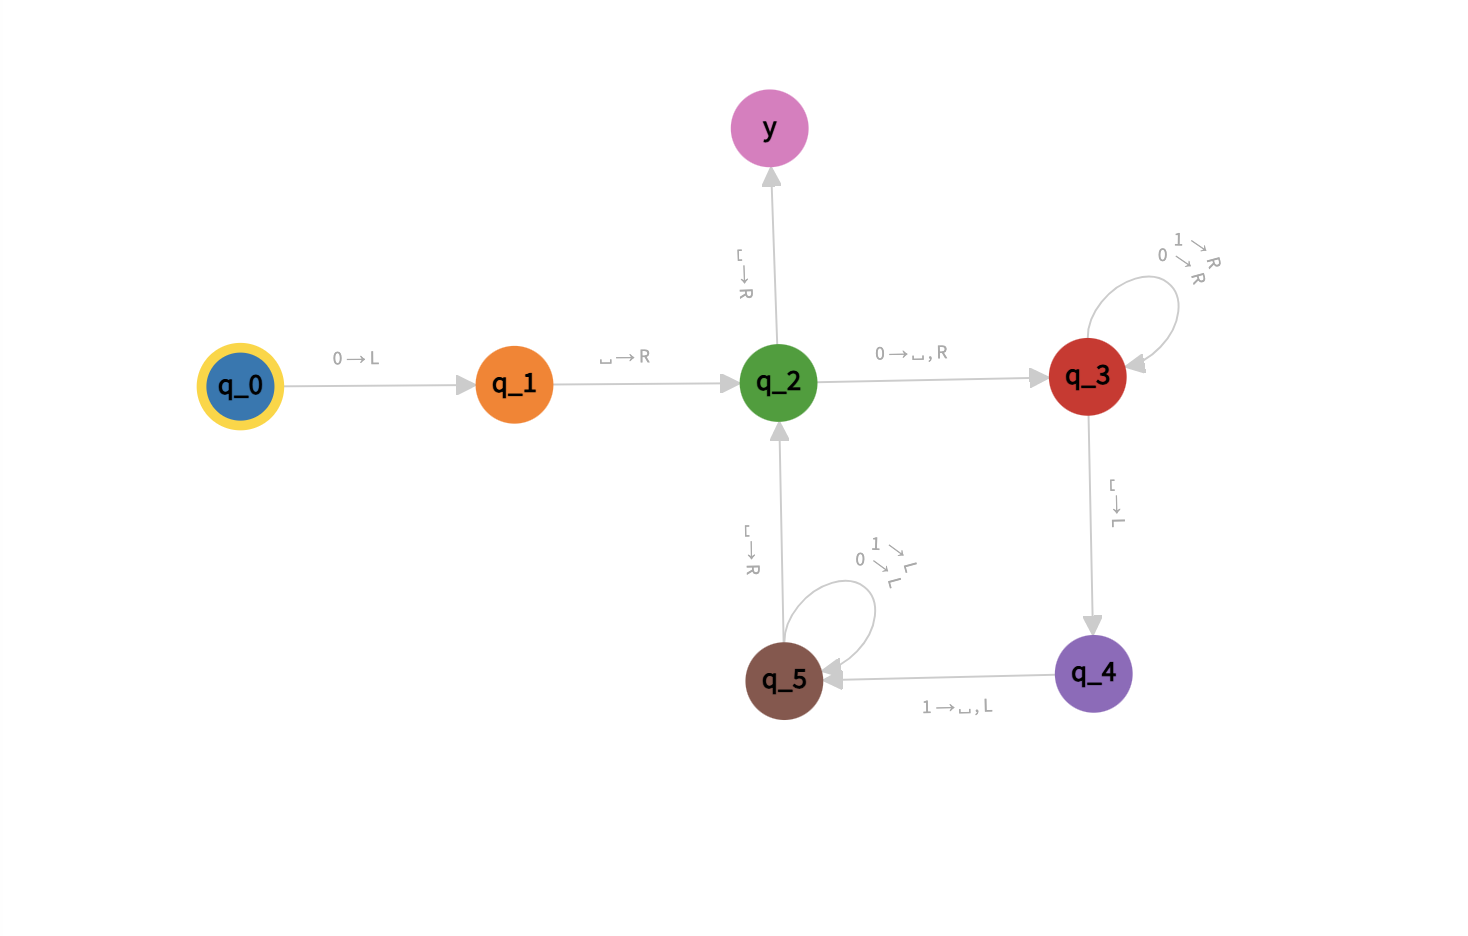
\includegraphics[width=\textwidth]{TM1.1}

In the first Turing machine the start state is $q_0$.
The states $q_0$ and $q_1$ are placed only to make sure that the machine doesn't accept the empty string, as $N \geq 1$.
The state $q_2$ deletes the symbol $0$ in the initial position, moves the head to the right and the machine goes to the state $q_3$.
The state $q_3$ makes the head go left until the first $\sqcup$ read, moves the head to the left and the machine goes to the state $q_4$.
The state $q_4$ deletes the symbol $1$ in the final position, moves the head to the left and the machine goes to the state $q_5$.
The state $q_5$ makes the head go left until the first $\sqcup$ read, moves the head to the left and the machine goes to the state $q_2$.
When the string is empty and the machine is in the state $q_2$, the machine accepts the input string and halts in the state $y$.

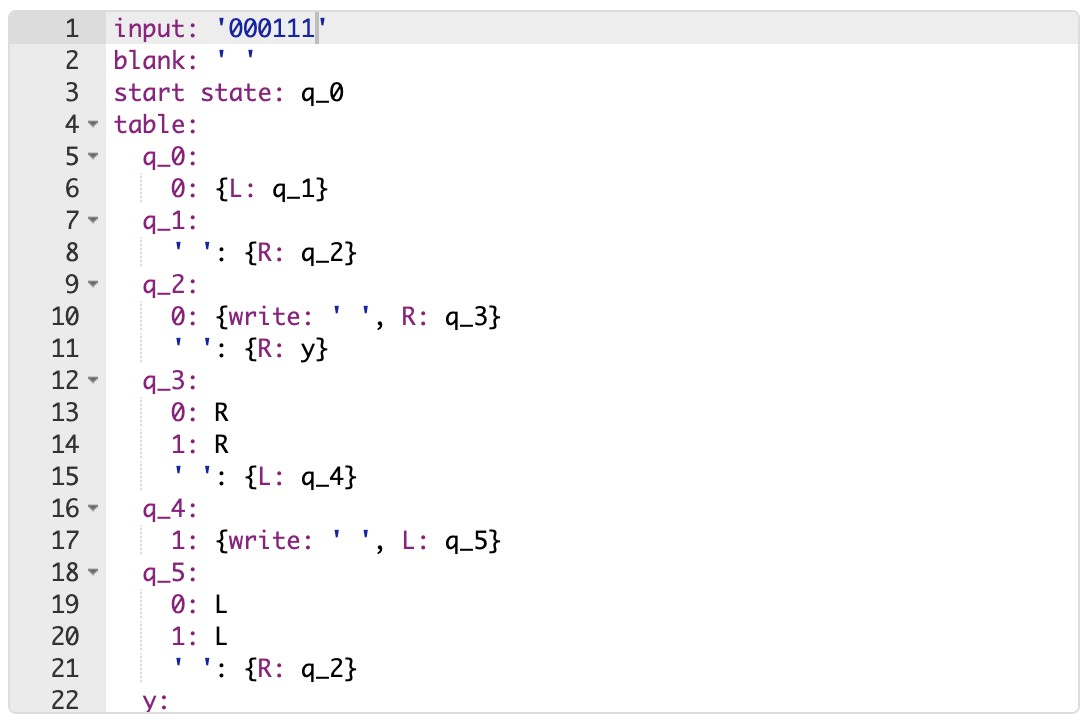
\includegraphics[width=\textwidth]{TM1.2}

\begin{changemargin}{1.77 cm}{0 cm}
\texttt
{
\\
input: '0001110' \\
blank: ' ' \\
start state: q\_0 \\
table: \\
  q\_0: \\
    0: \{L: q\_1\} \\
  q\_1: \\
    ' ': \{R: q\_2\} \\
  q\_2: \\
    0: \{write: ' ', R: q\_3\} \\
    ' ': \{R: y\} \\
  q\_3: \\
    0: R \\
    1: R \\
    ' ': \{L: q\_4\} \\
  q\_4: \\
    1: \{write: ' ', L: q\_5\} \\
  q\_5: \\
    0: L \\
    1: L \\
    ' ': \{R: q\_2\} \\
  y: \\
}
\end{changemargin}
\newpage
\begin{center}
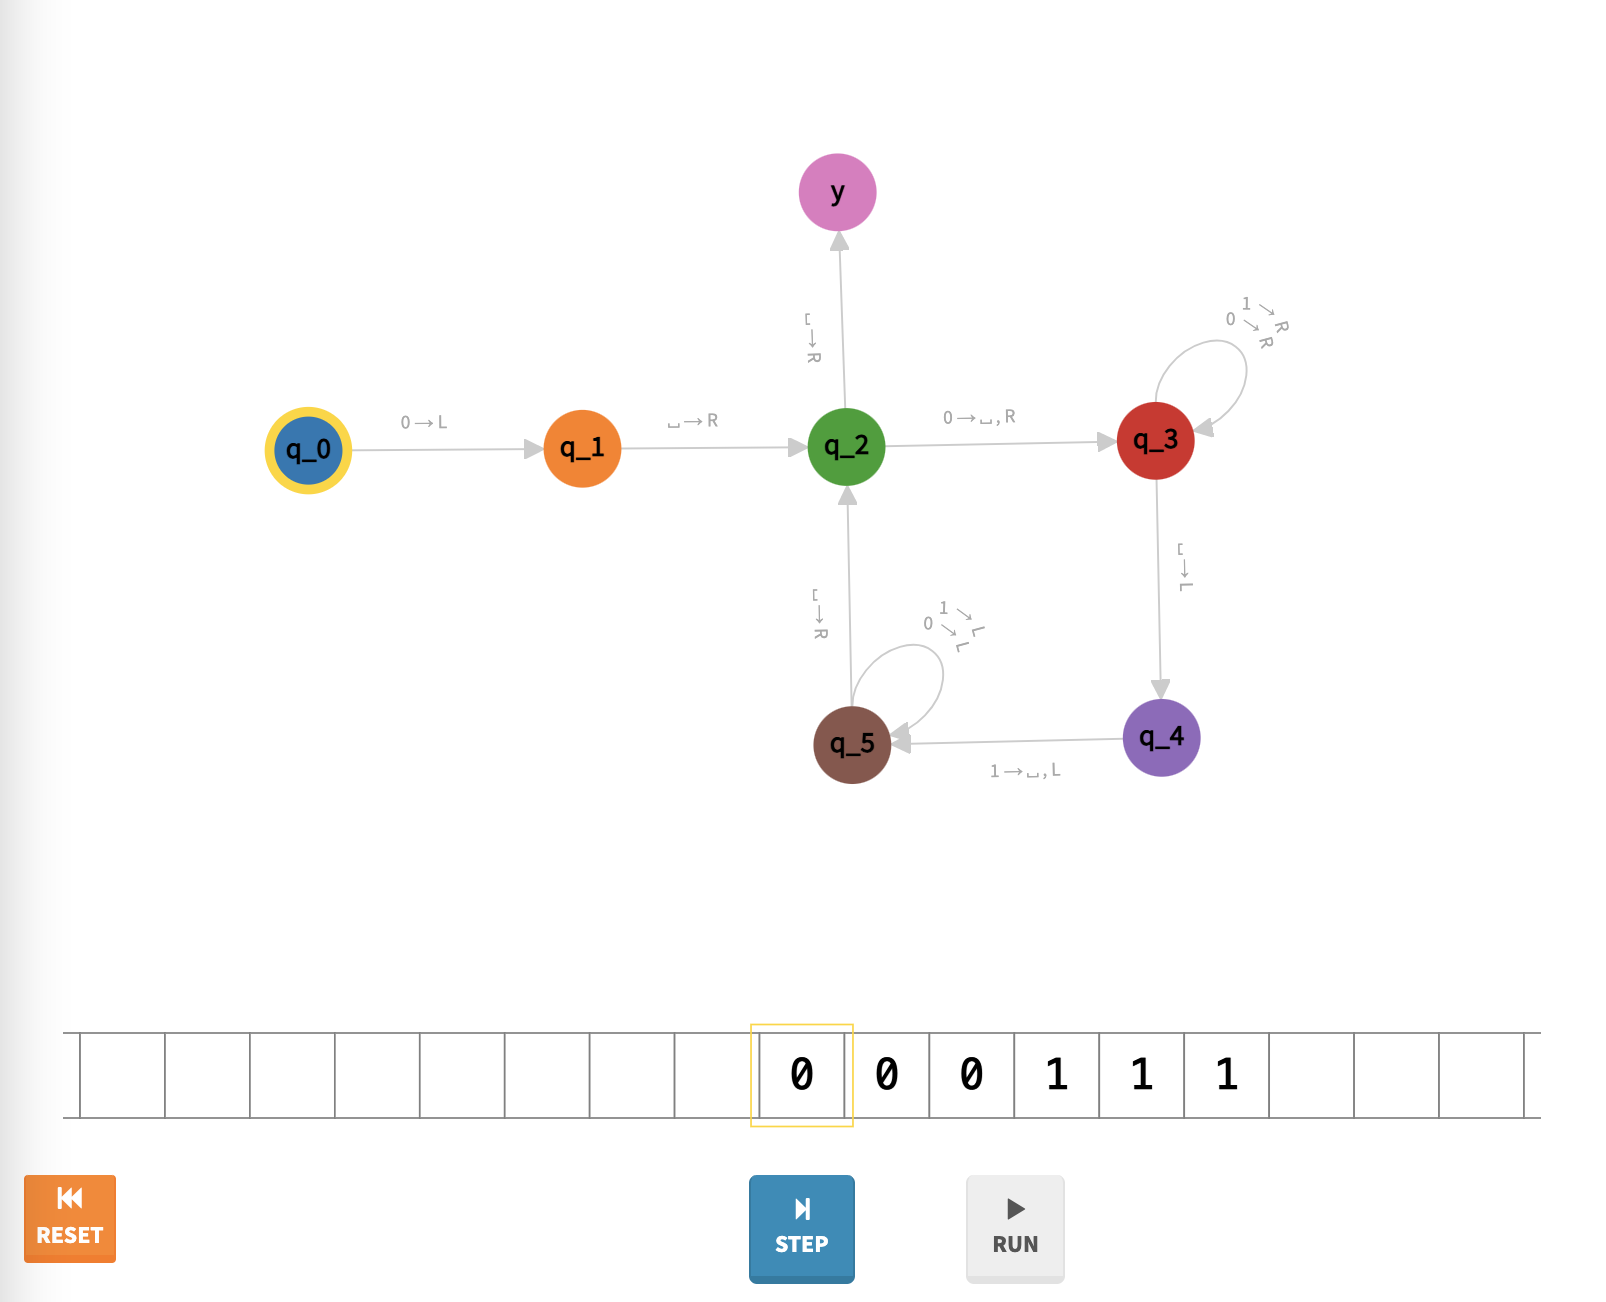
\includegraphics[width=\textwidth]{TM1.3}
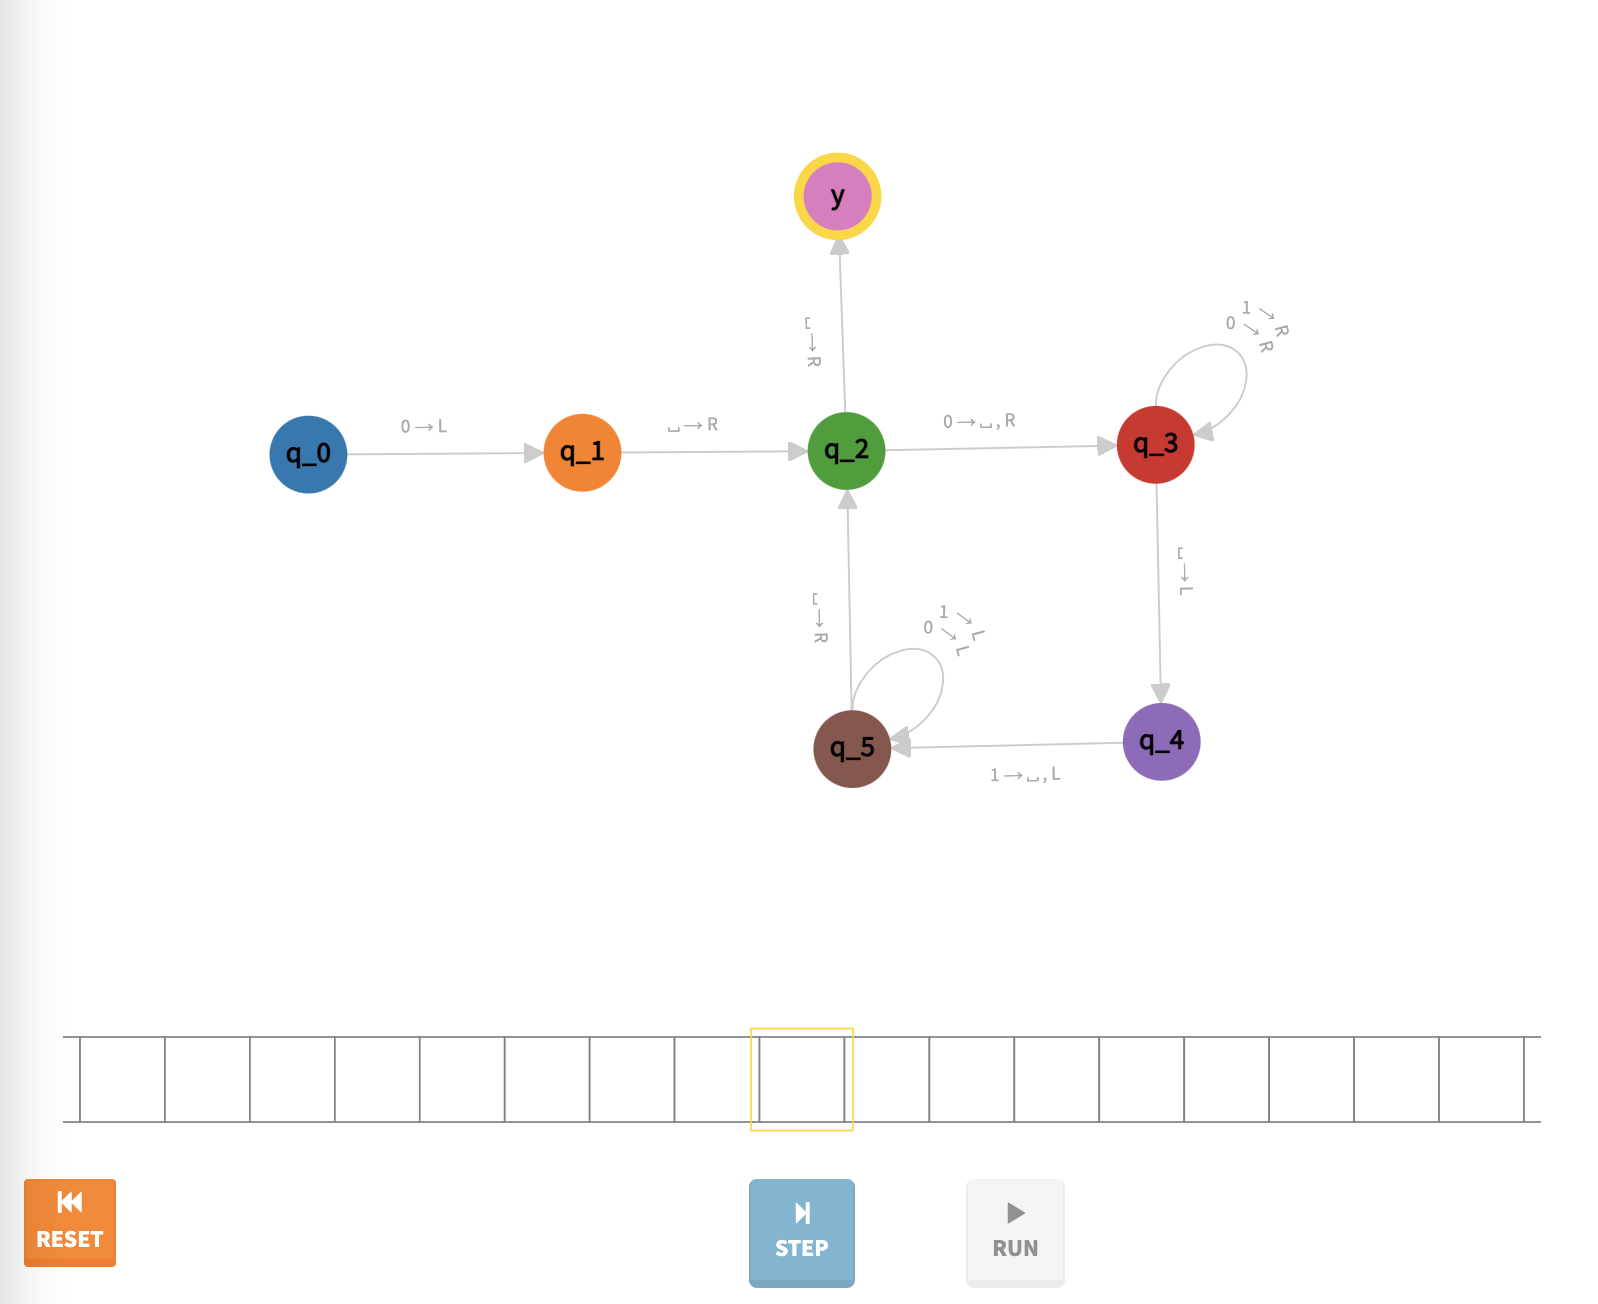
\includegraphics[width=\textwidth]{TM1.4}
\end{center}
\newpage
\begin{center}
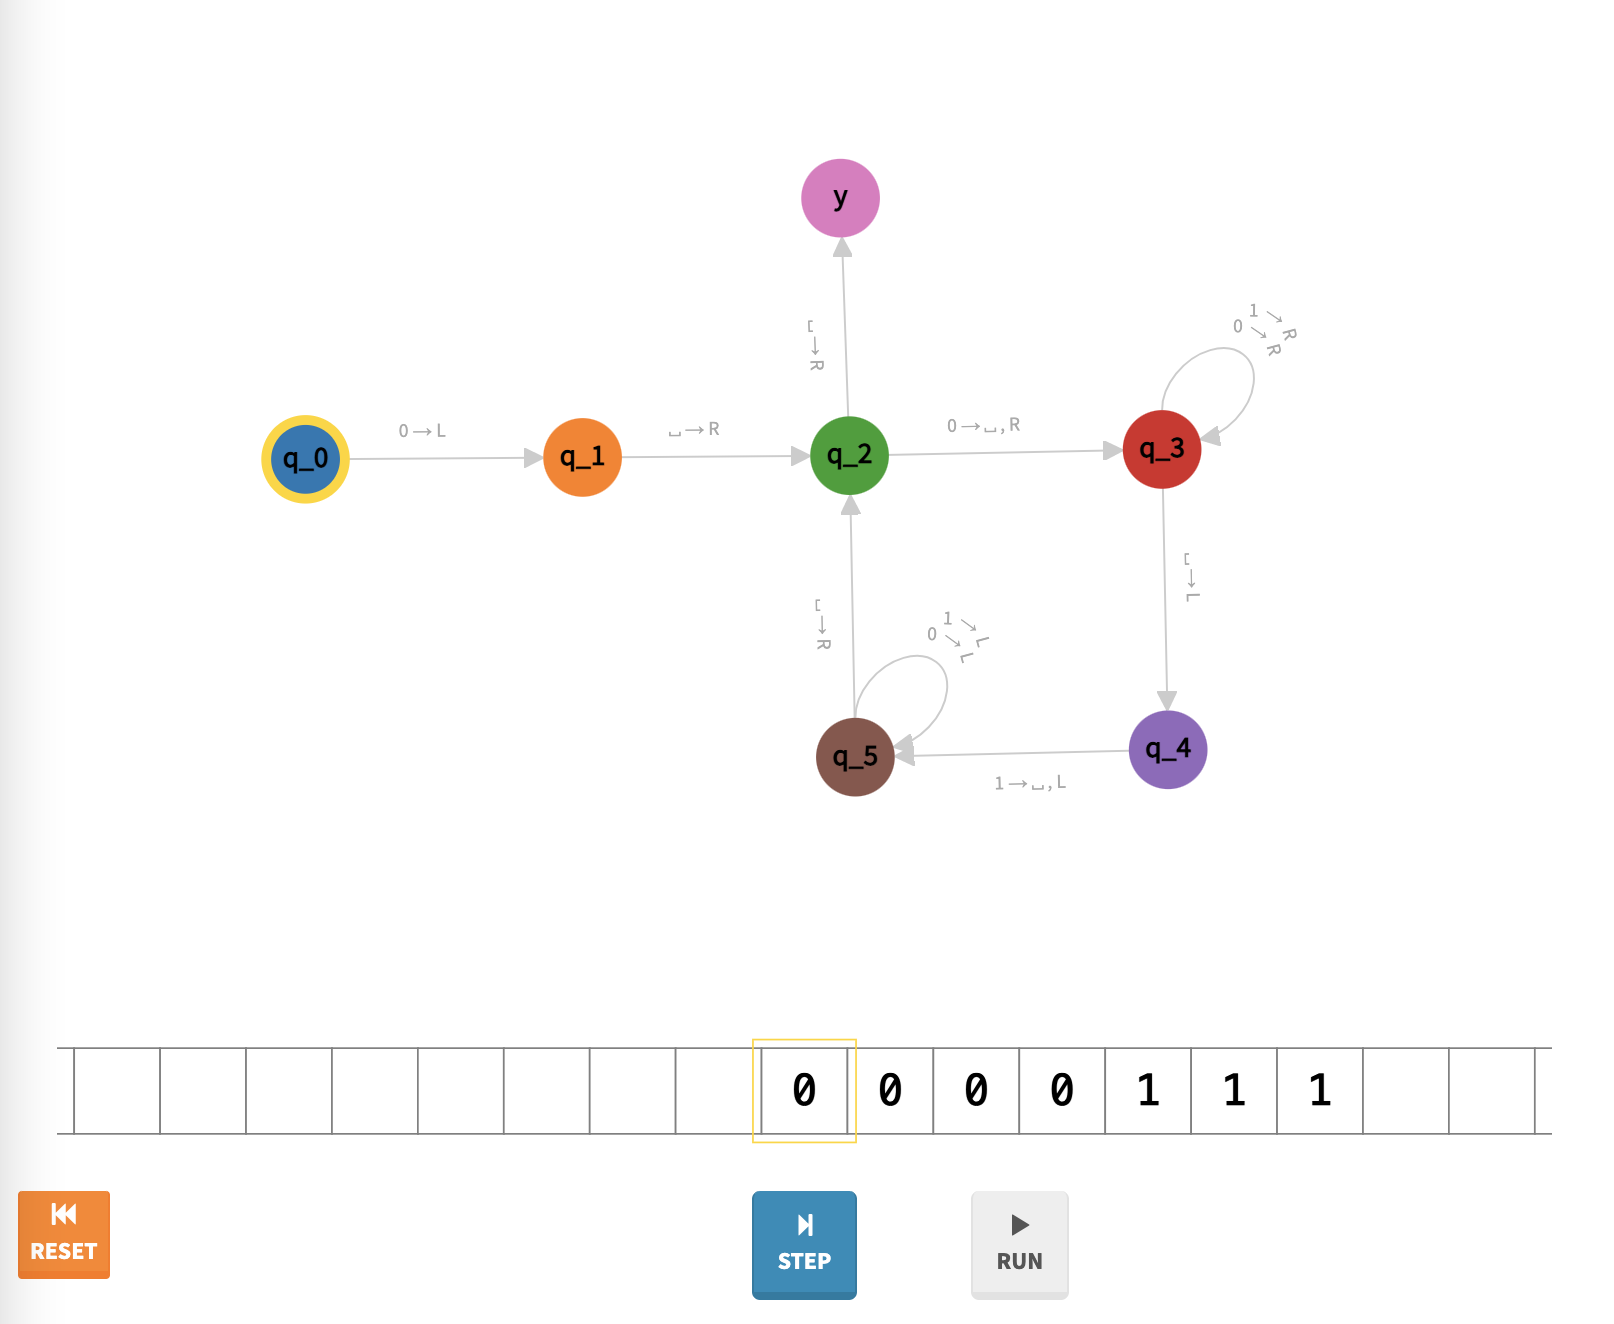
\includegraphics[width=\textwidth]{TM1.5}
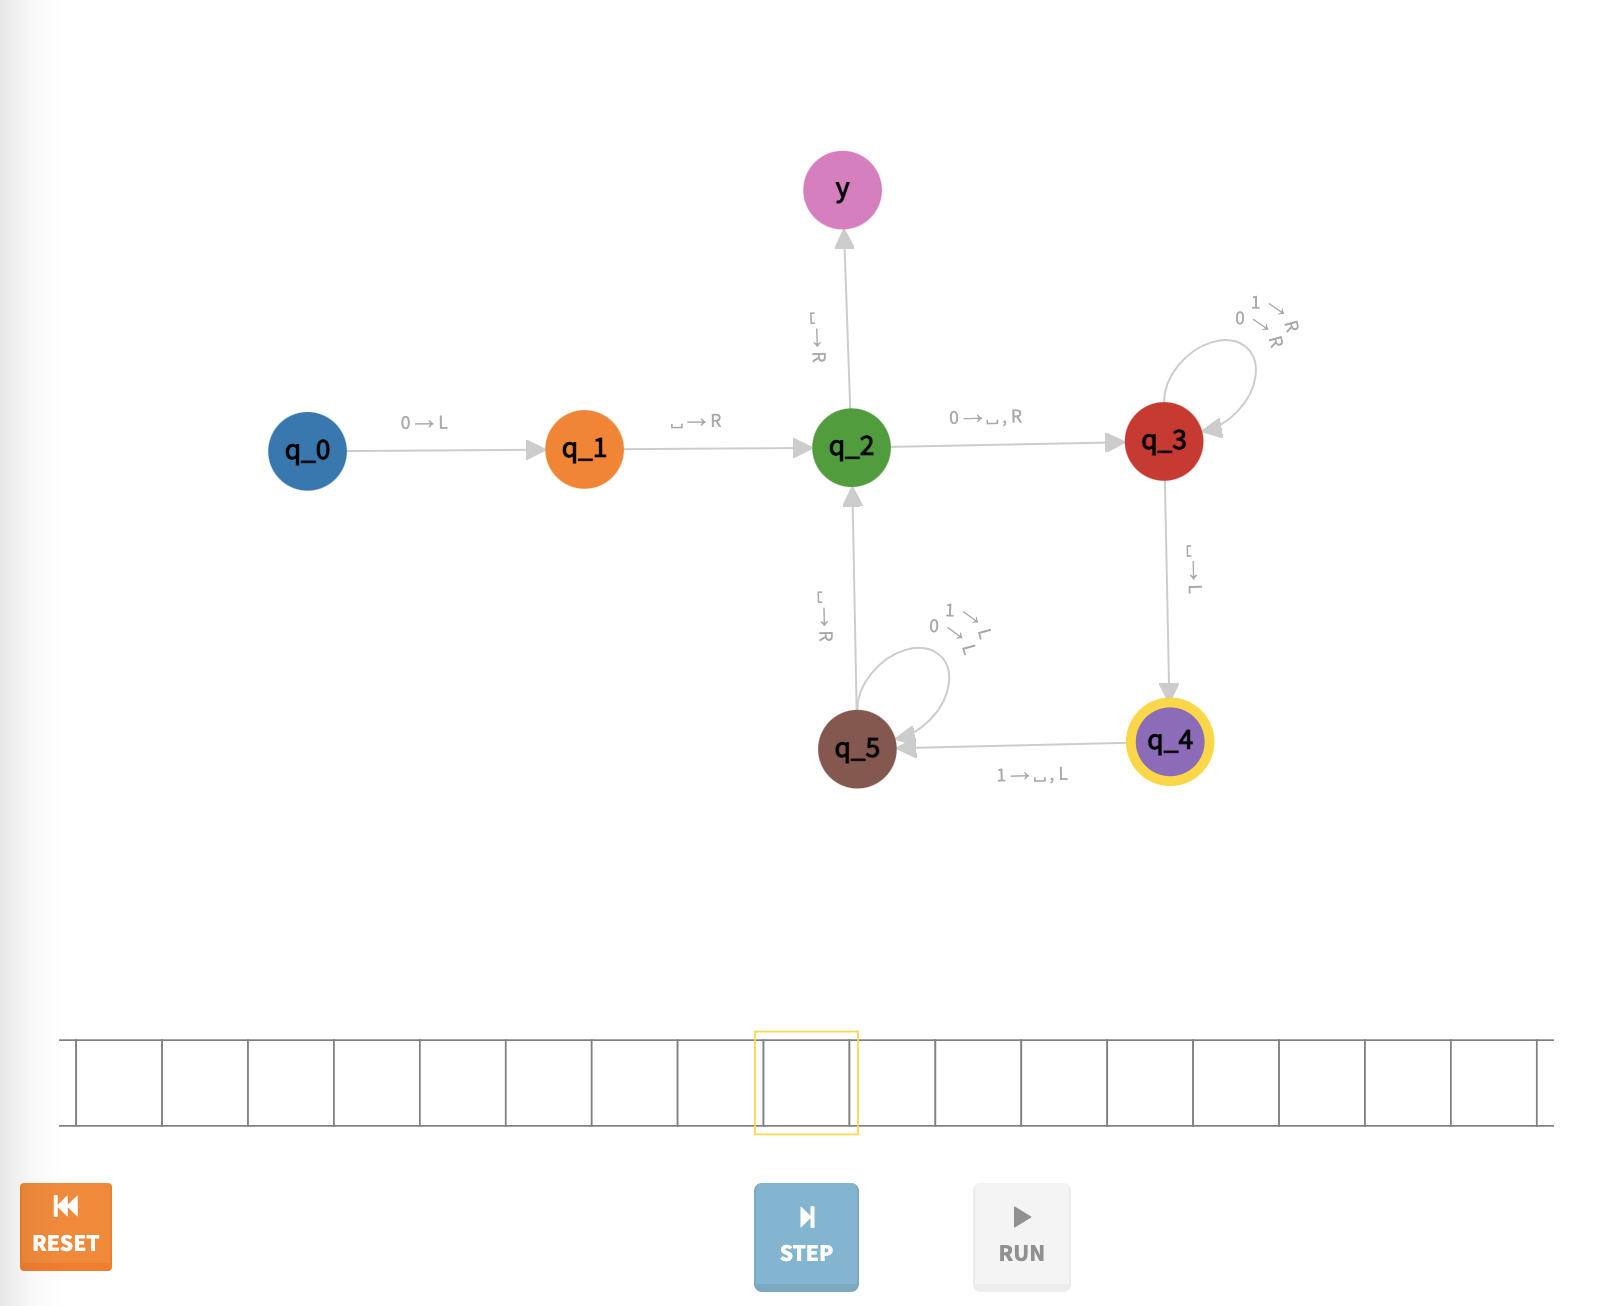
\includegraphics[width=\textwidth]{TM1.6}
\end{center}
\newpage
\begin{center}
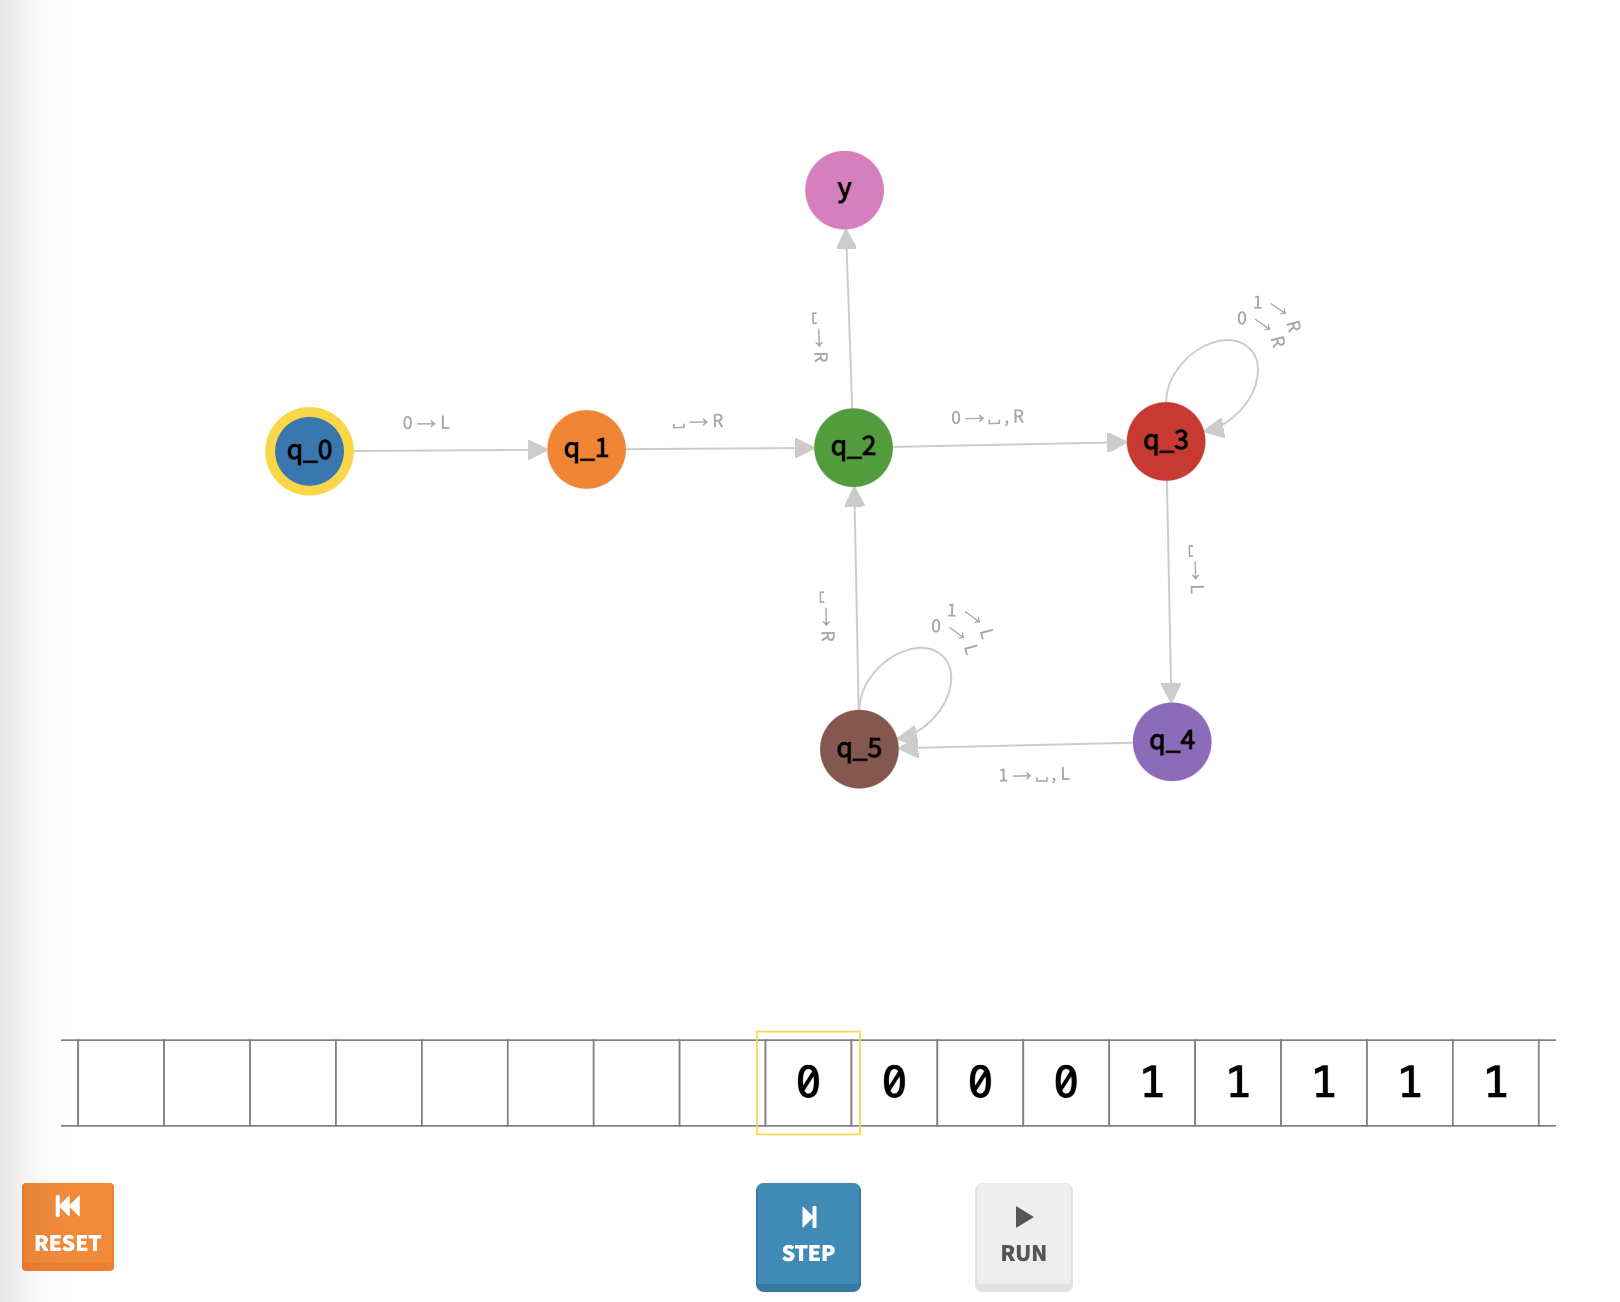
\includegraphics[width=\textwidth]{TM1.7}
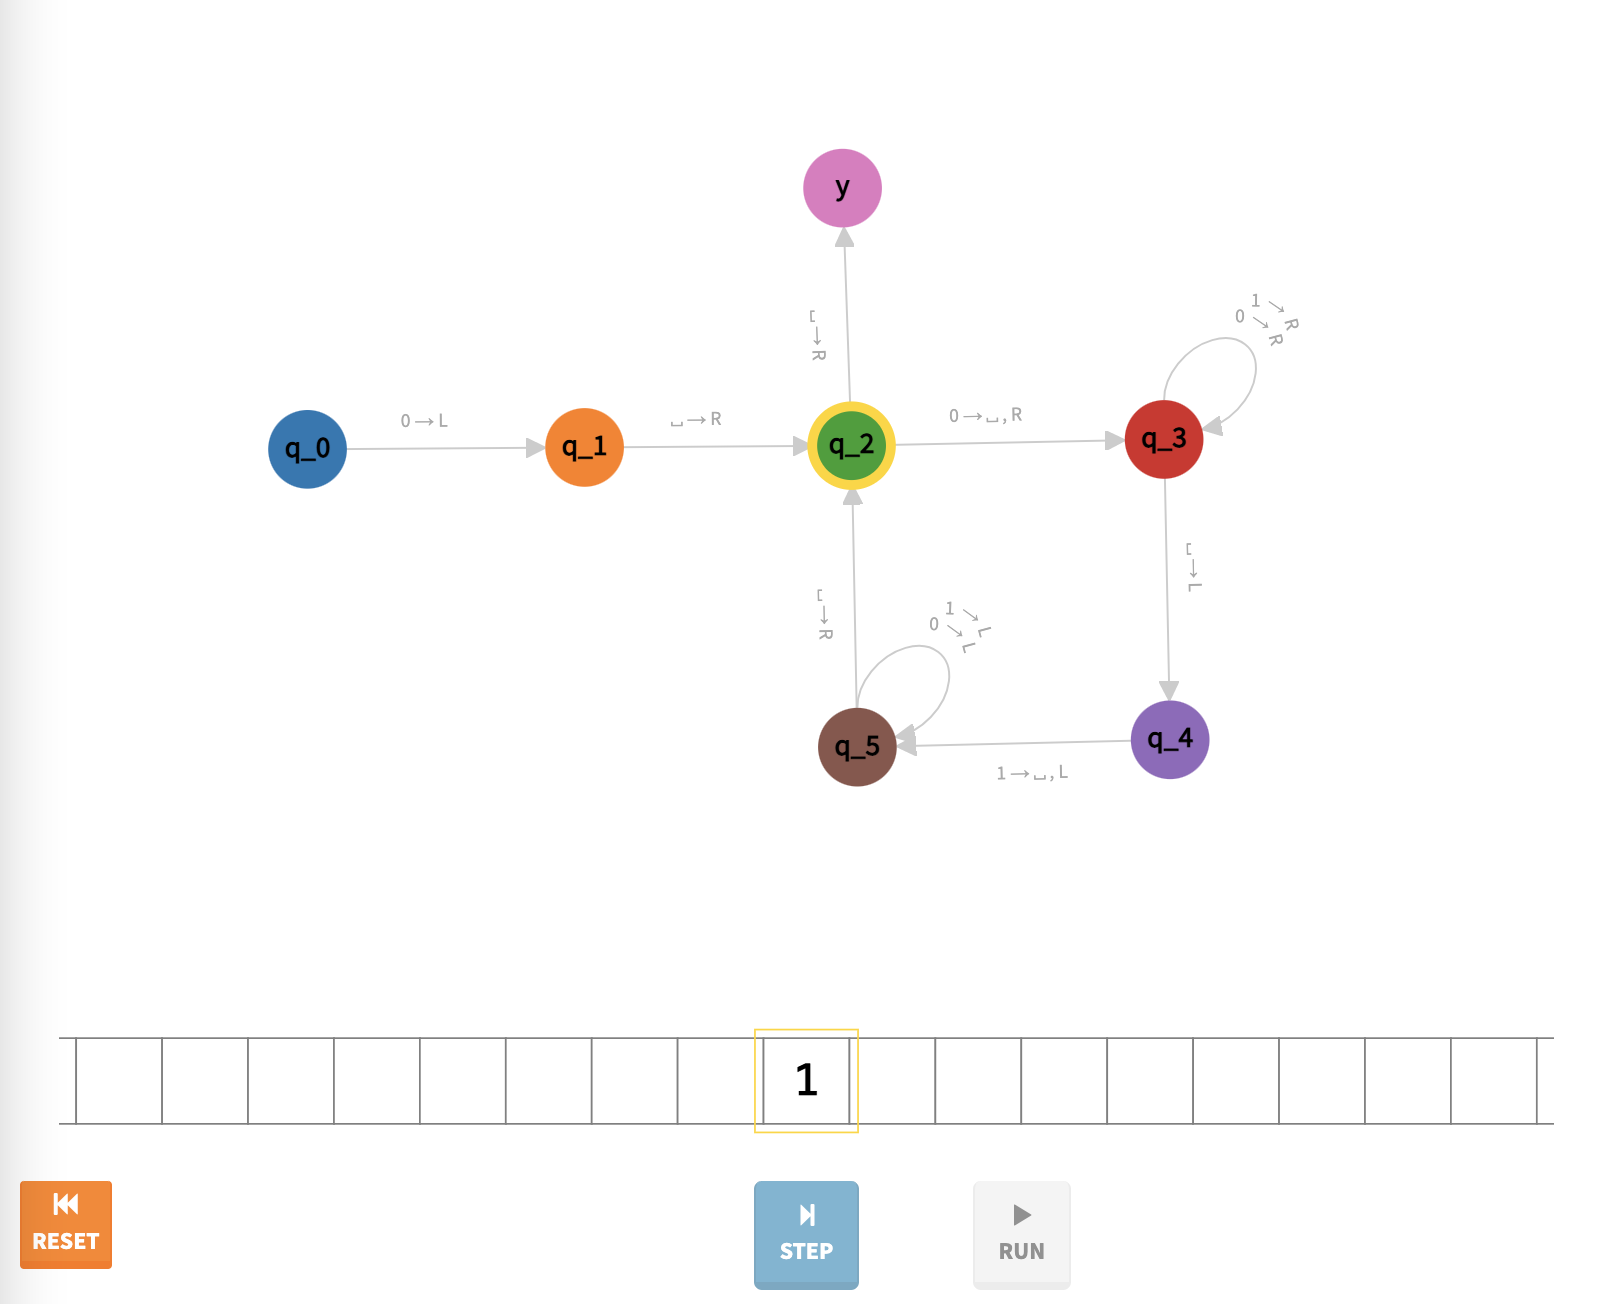
\includegraphics[width=\textwidth]{TM1.8}
\end{center}
\newpage
\begin{center}
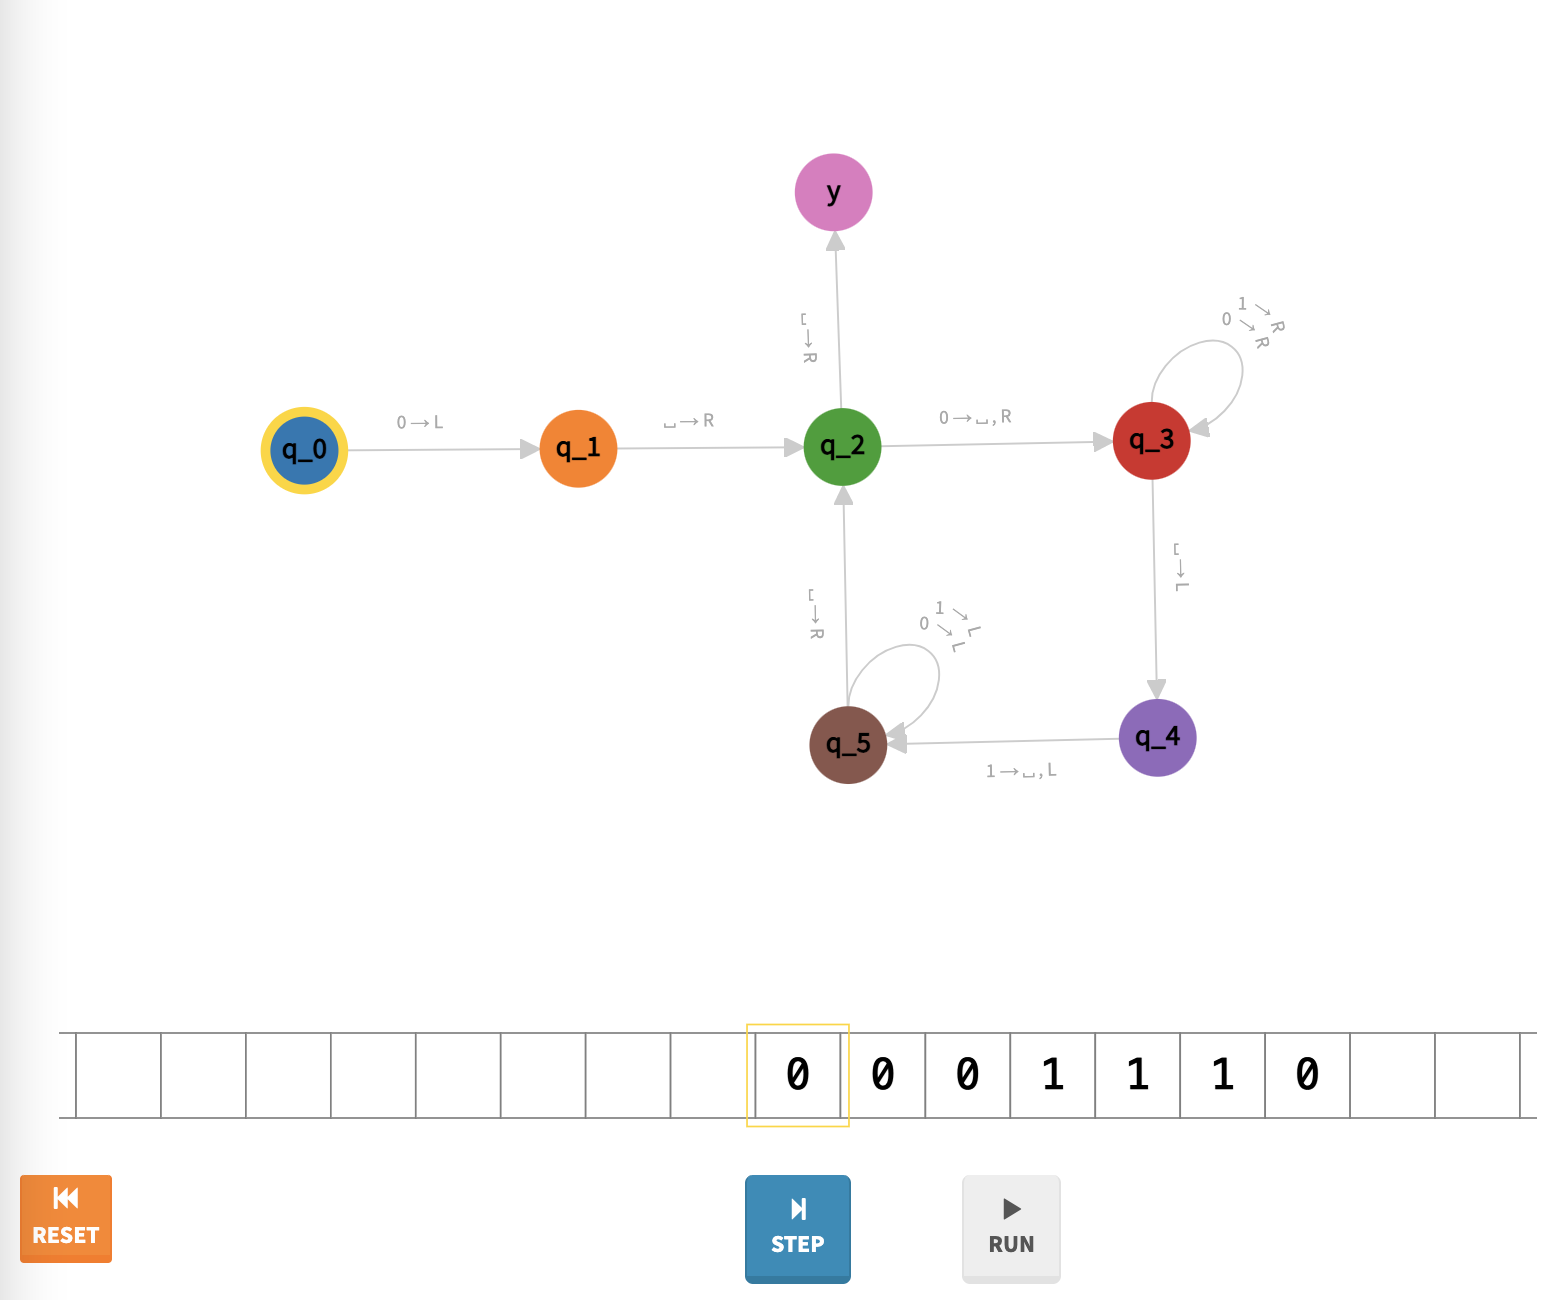
\includegraphics[width=\textwidth]{TM1.9}
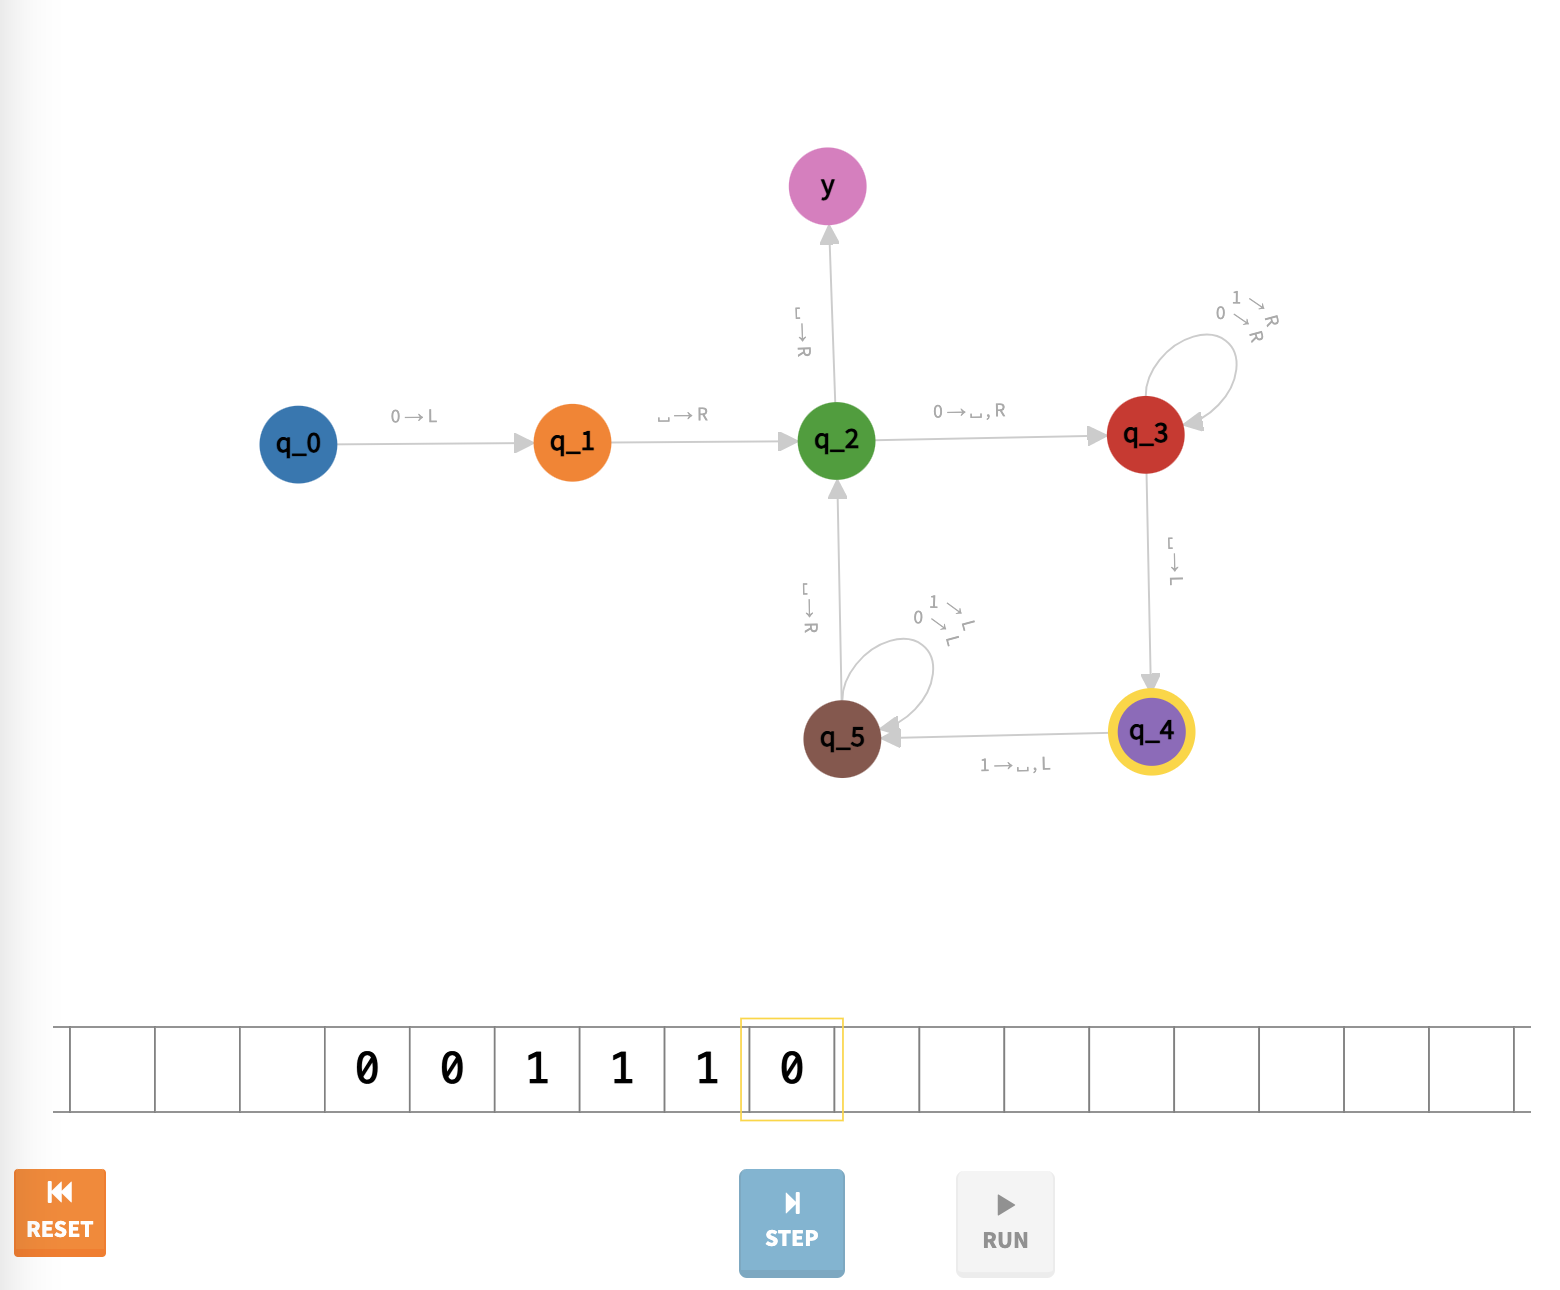
\includegraphics[width=\textwidth]{TM1.10}
\end{center}
\newpage
\begin{center}
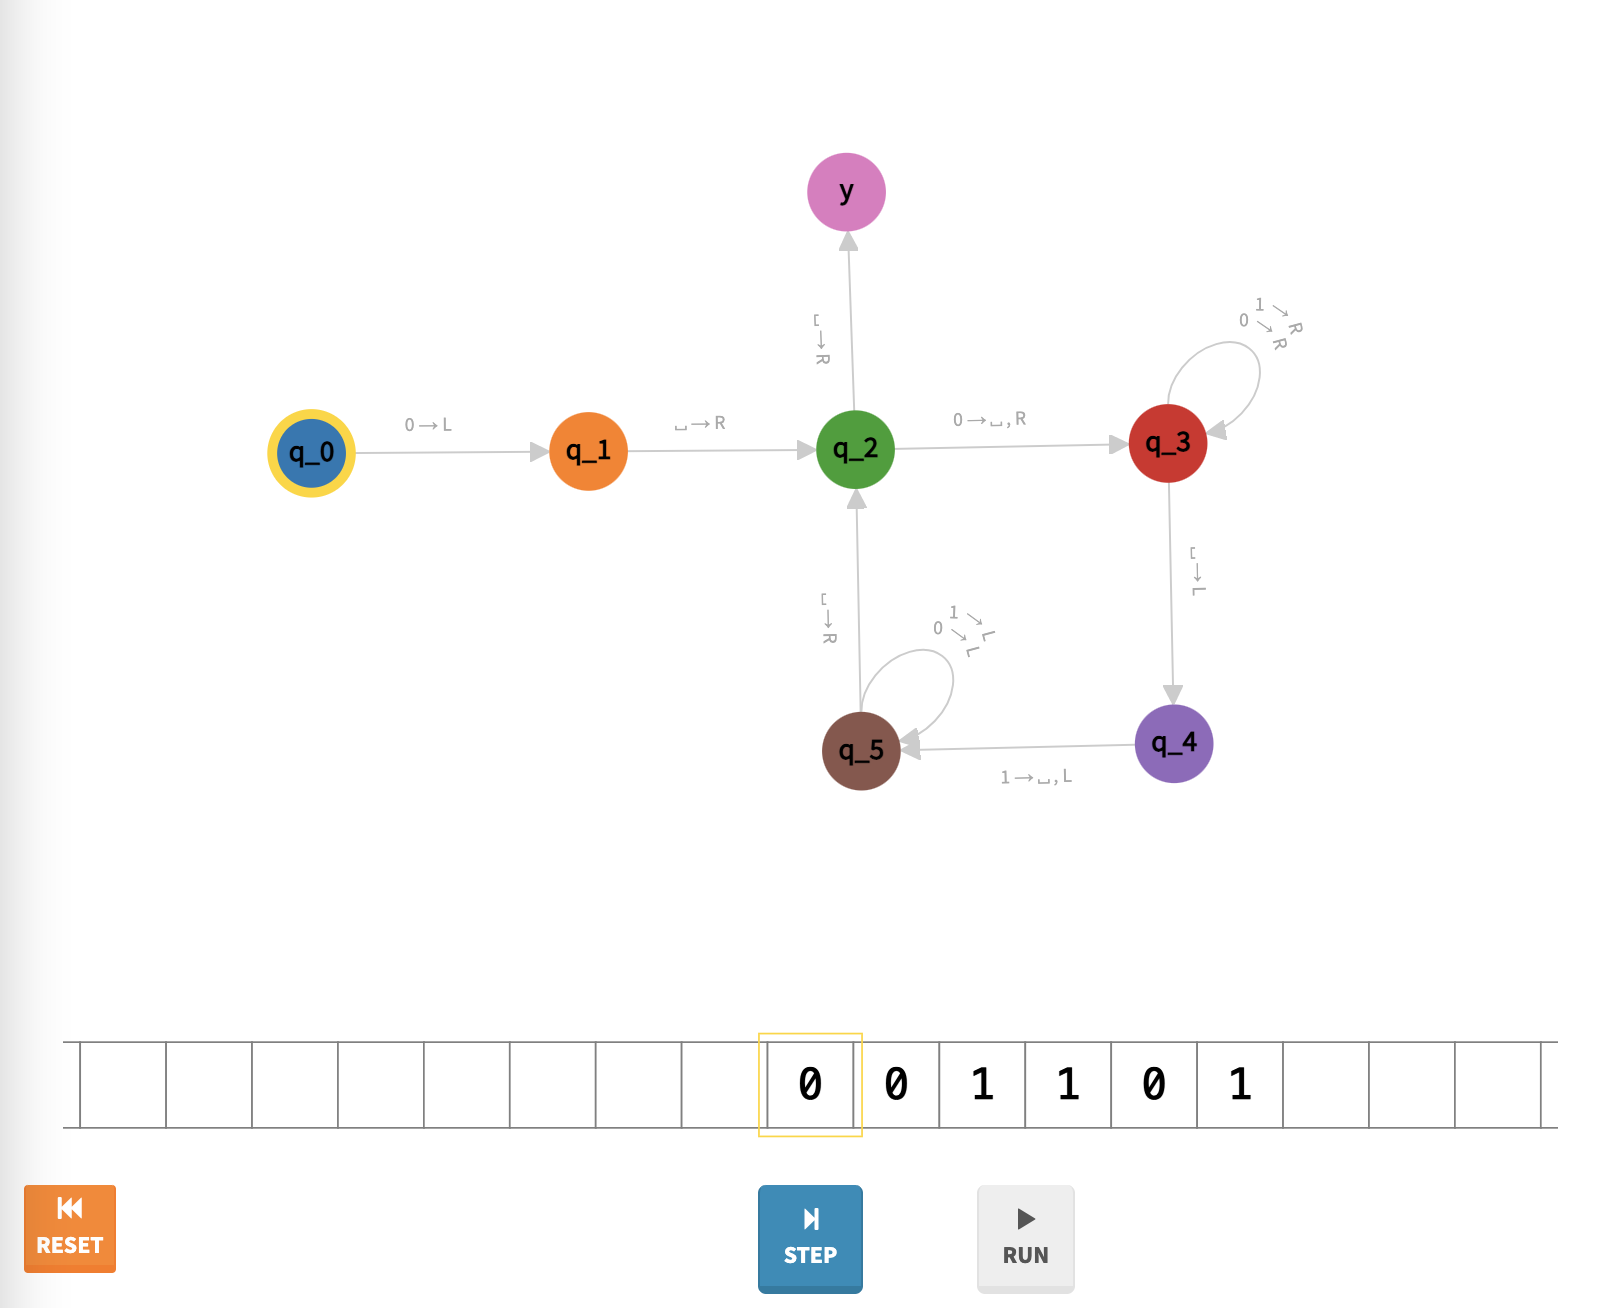
\includegraphics[width=\textwidth]{TM1.11}
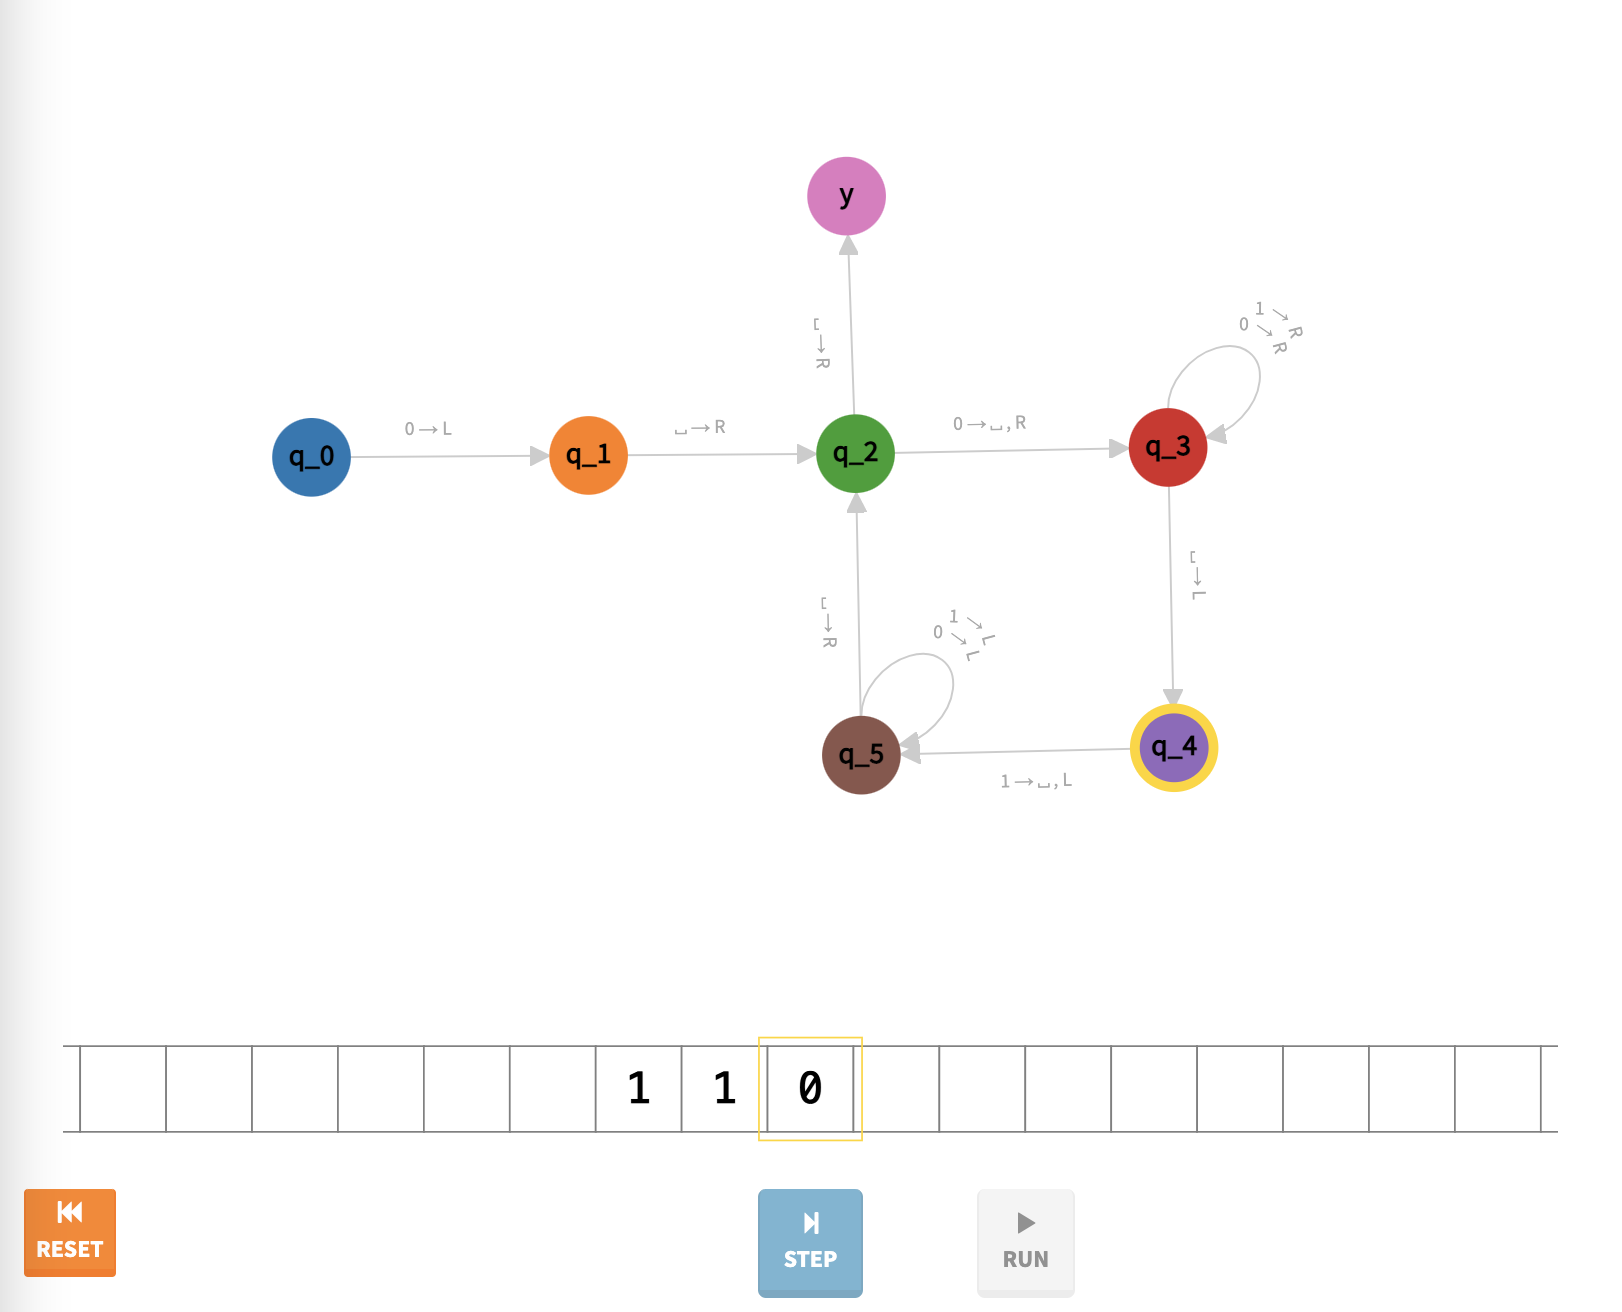
\includegraphics[width=\textwidth]{TM1.12}
\end{center}
\newpage
\begin{center}
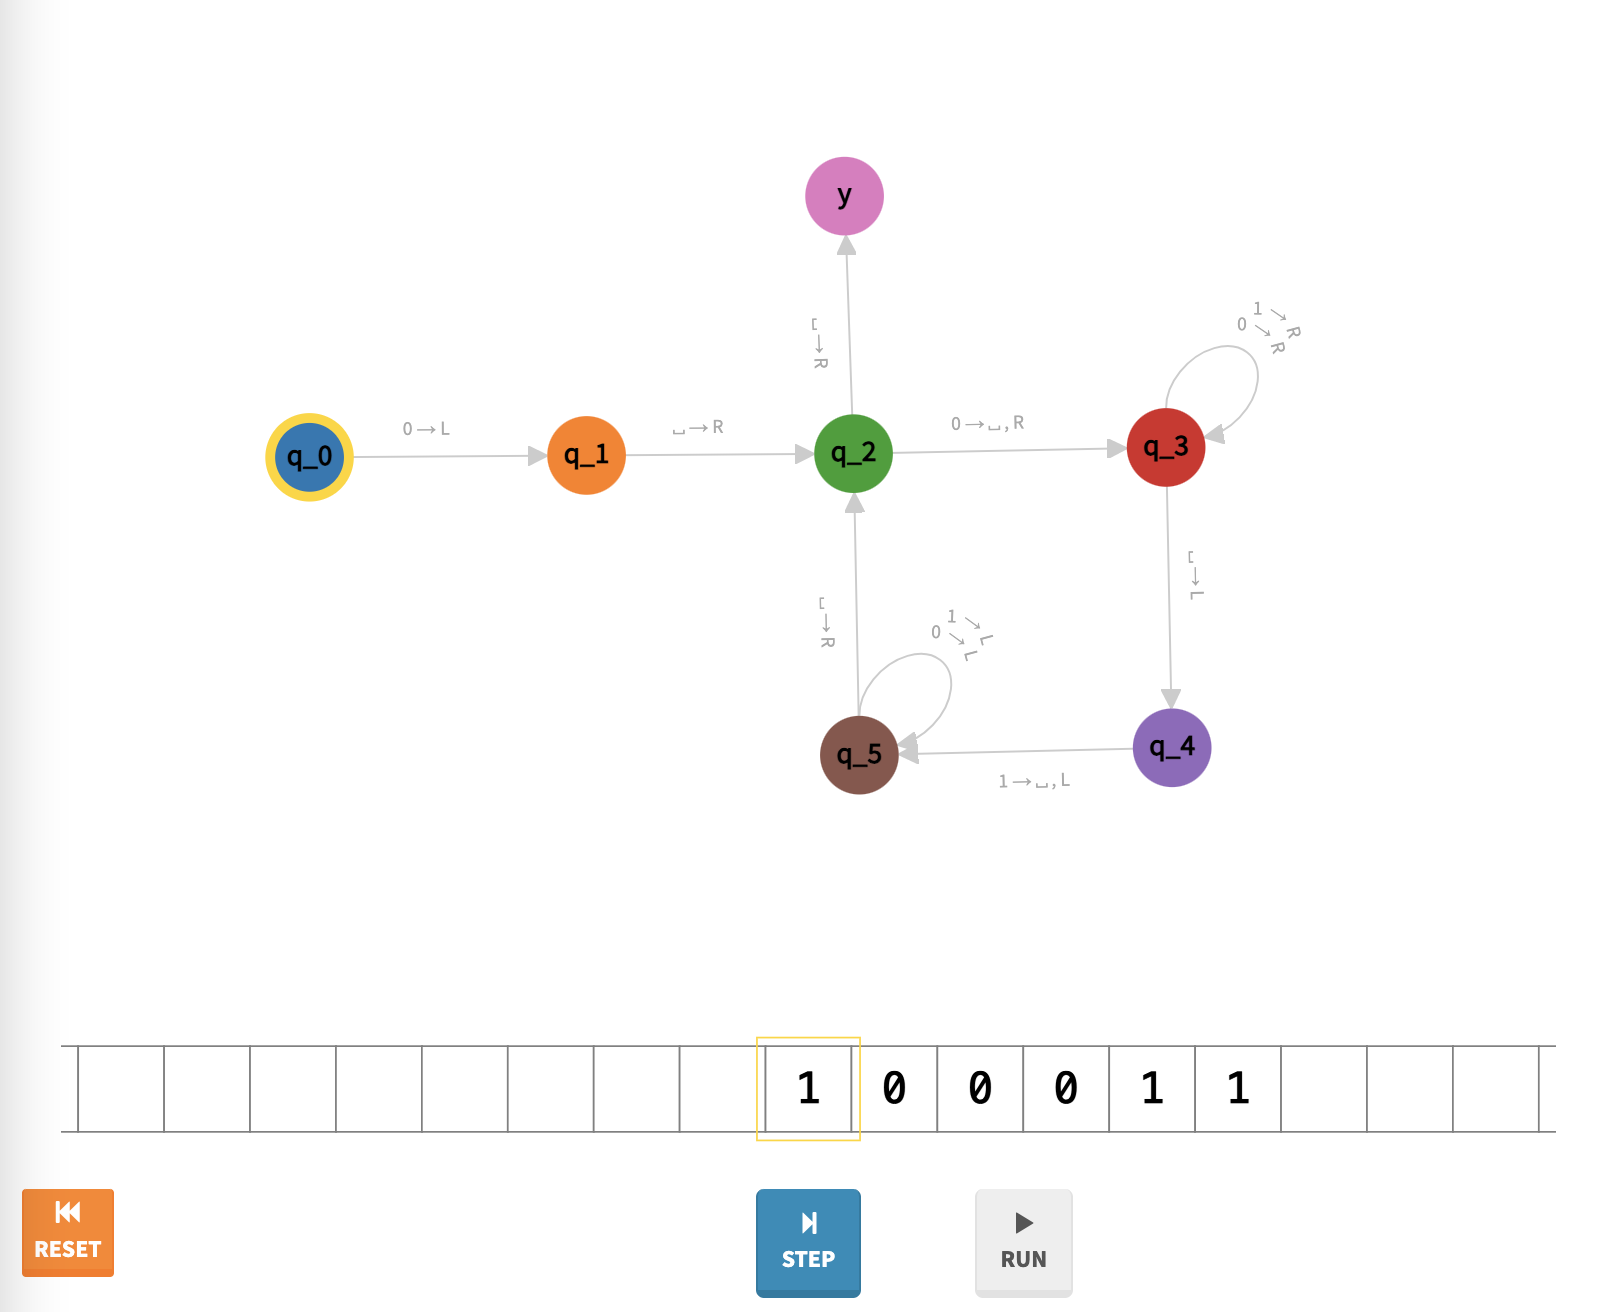
\includegraphics[width=\textwidth]{TM1.13}
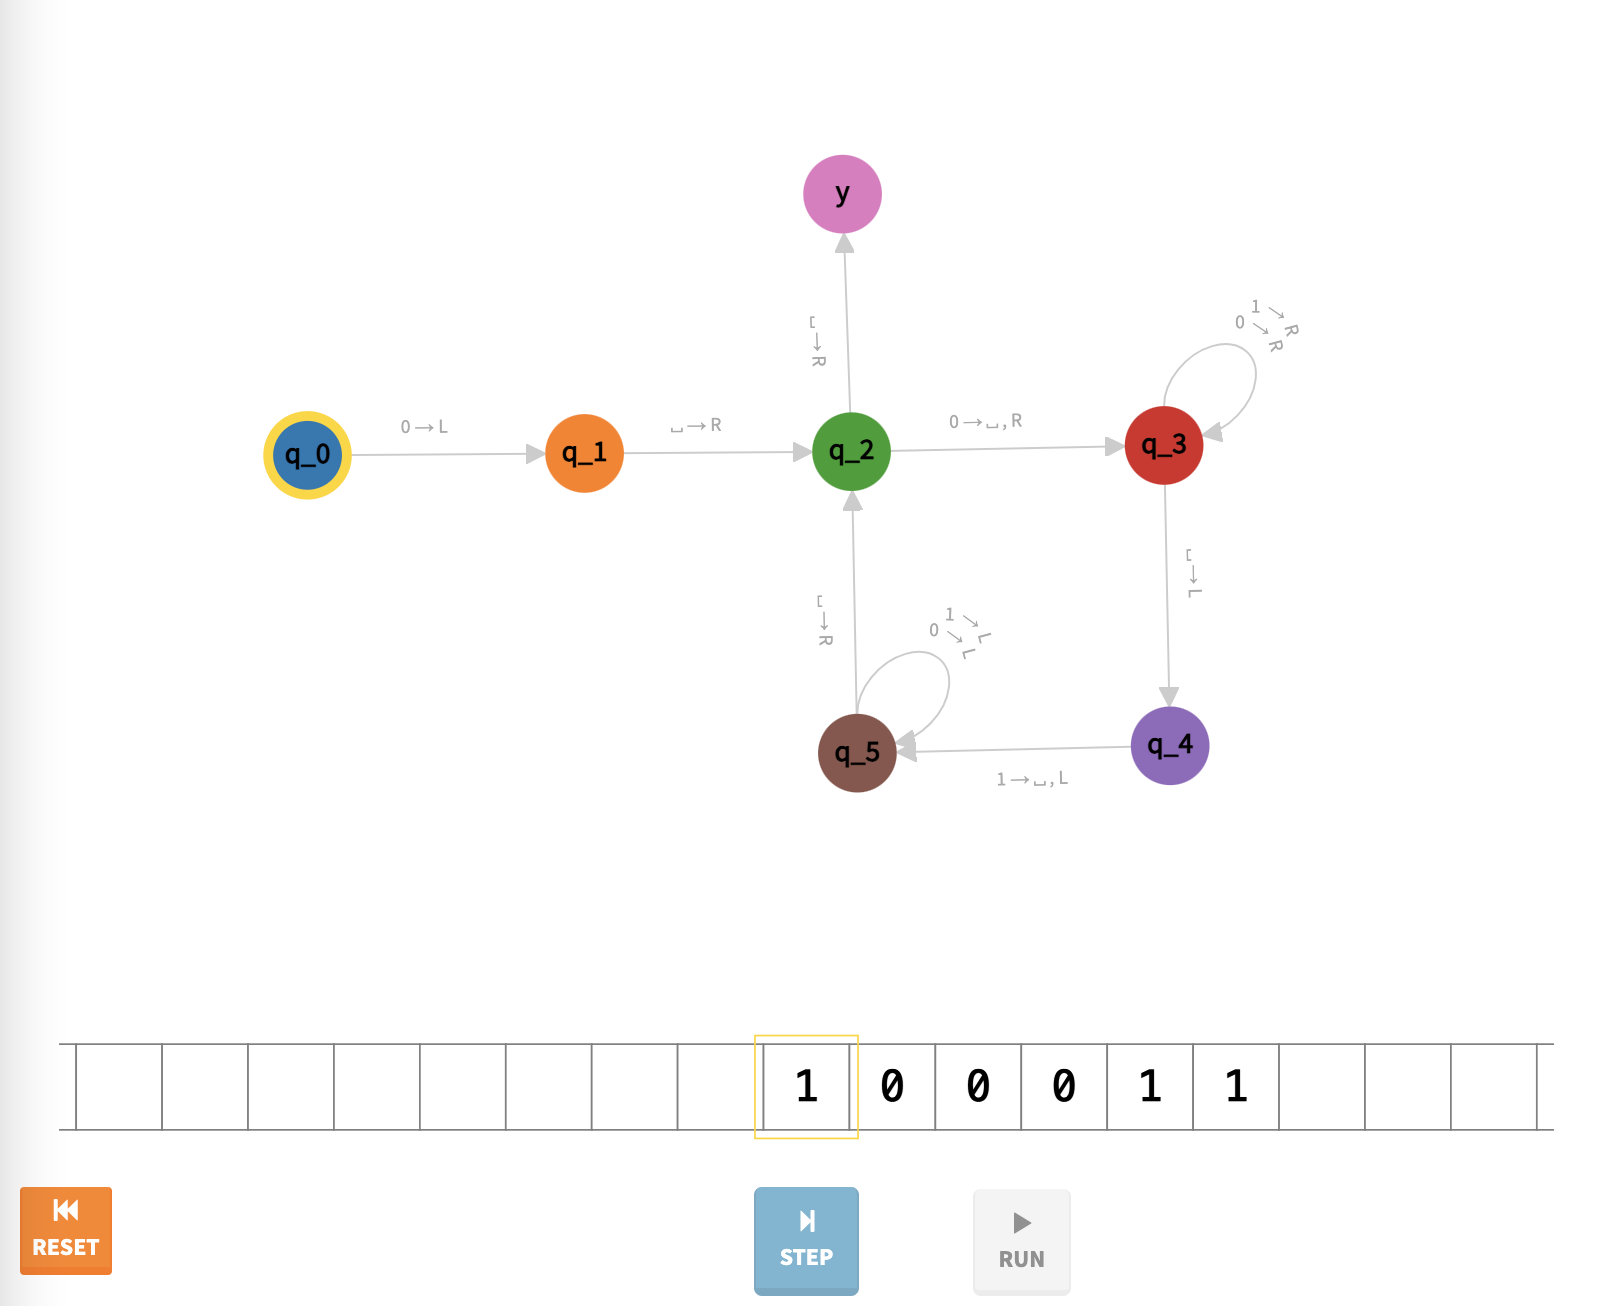
\includegraphics[width=\textwidth]{TM1.14}
\end{center}

\newpage

\section*{Answer 2}

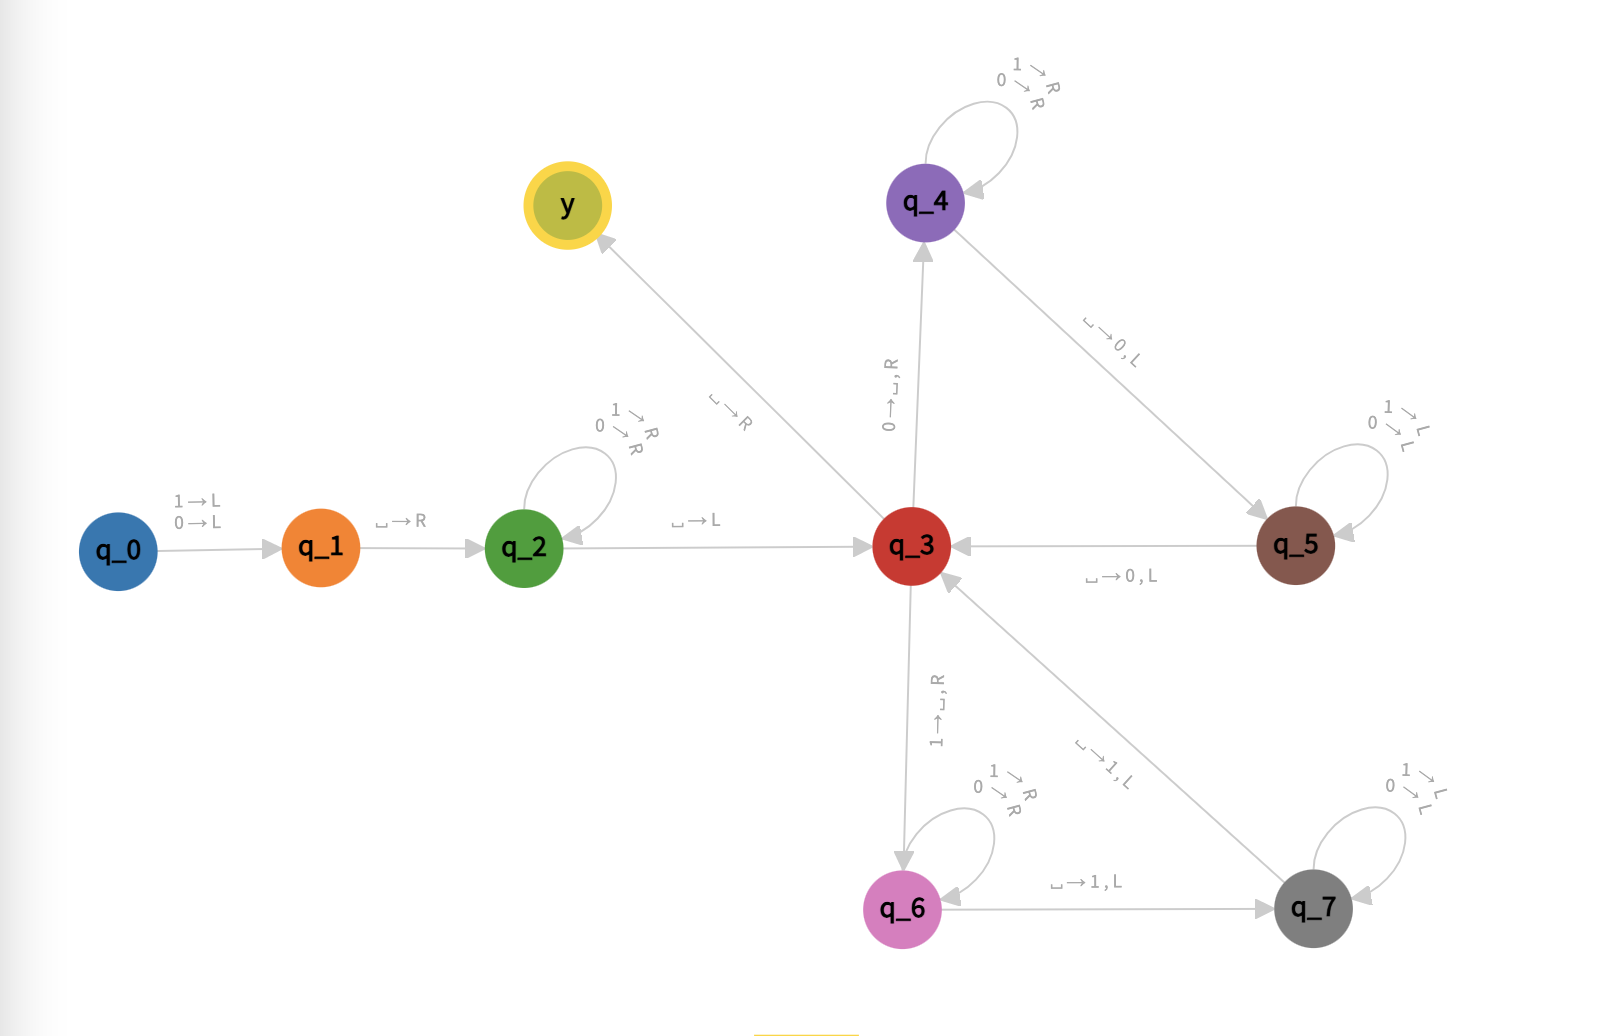
\includegraphics[width=\textwidth]{TM2.1}

In the second Turing machine the start state is $q_0$.
The states $q_0$ and $q_1$ are placed only to make sure that the machine doesn't accept the empty string, as $e \notin \{0,1\}^+$.
The state $q_2$ makes the head go right until the first $\sqcup$ read, moves the head to the left and the machine goes to the state $q_3$.
The state $q_3$ deletes the symbol $0$ (or $1$), moves the head to the right and the machine goes to the state $q_4$ (or $q_6$).
The state $q_4$ (or $q_6$) moves the head to the right until the first $\sqcup$ read, writes the symbol $0$ (or $1$), moves the head to the left and the machine goes to the state $q_5$ (or $q_7$).
The state $q_5$ (or $q_7$) moves the head to the left until the first $\sqcup$ seen, writes the symbol $0$ (or $1$), and the machine goes the state $q_3$.
When the head reads $\sqcup$ and the machine is in the state $q_3$, the machine halts in the state $y$.

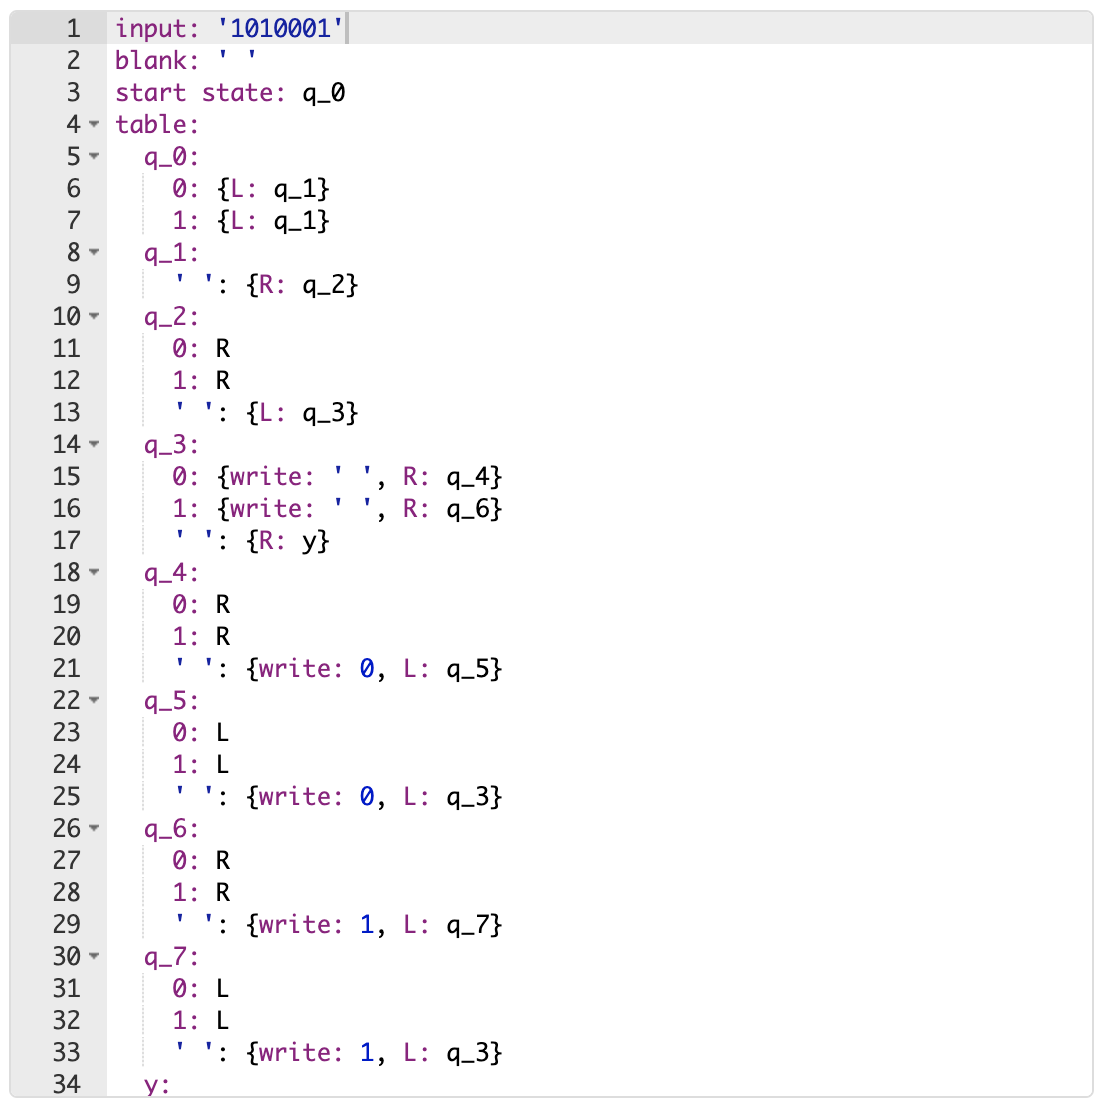
\includegraphics[width=\textwidth]{TM2.2}

\newpage

\begin{changemargin}{1.77 cm}{0 cm}
\texttt
{
\\
input: '1011' \\
blank: ' ' \\
start state: q\_0 \\
table: \\
  q\_0: \\
    0: {L: q\_1} \\
    1: {L: q\_1} \\
  q\_1: \\
    ' ': {R: q\_2} \\
  q\_2: \\
    0: R \\
    1: R \\
    ' ': {L: q\_3} \\
  q\_3: \\
    0: {write: ' ', R: q\_4} \\
    1: {write: ' ', R: q\_6} \\
    ' ': {R: y} \\
  q\_4: \\
    0: R \\
    1: R \\
    ' ': {write: 0, L: q\_5} \\
  q\_5: \\
    0: L \\
    1: L \\
    ' ': {write: 0, L: q\_3} \\
  q\_6: \\
    0: R \\
    1: R \\
    ' ': {write: 1, L: q\_7} \\
  q\_7: \\
    0: L \\
    1: L \\
    ' ': {write: 1, L: q\_3} \\
  y: \\
}
\end{changemargin}
\newpage
\begin{center}
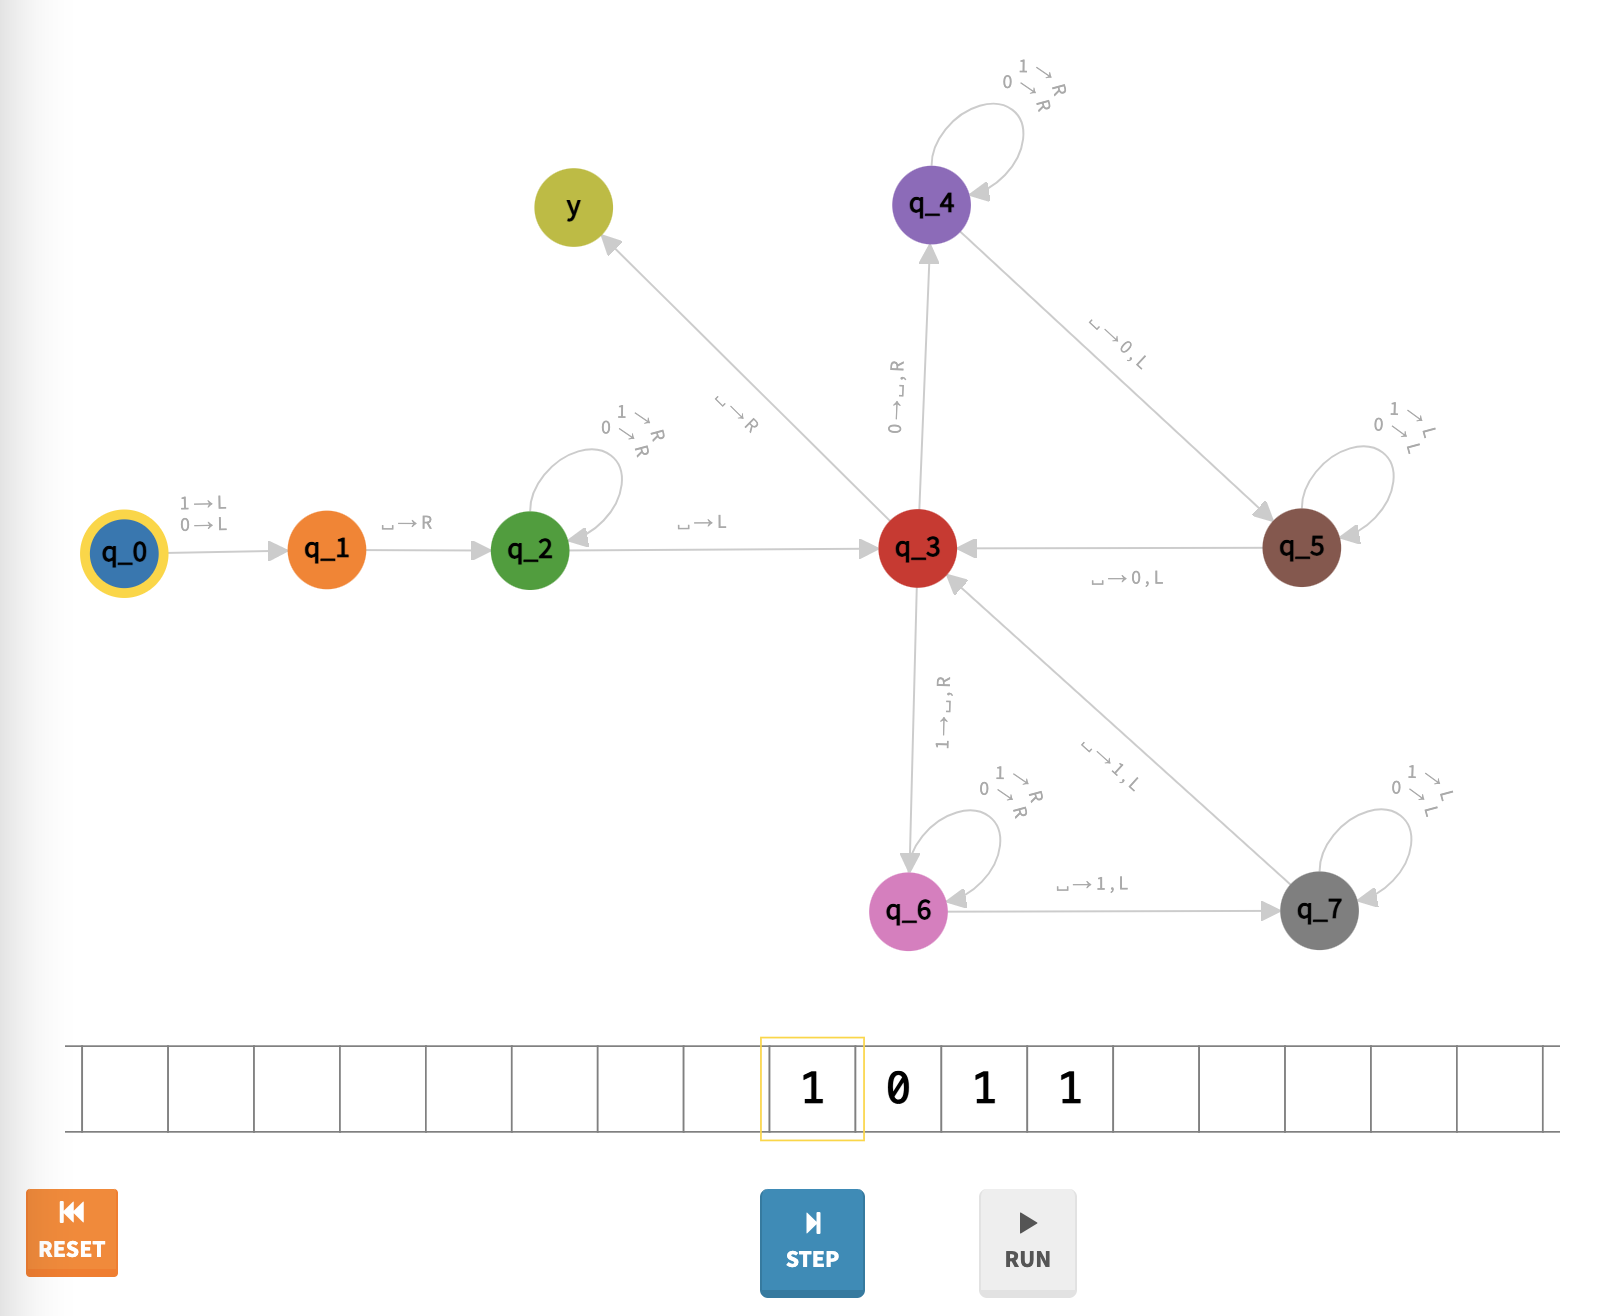
\includegraphics[width=\textwidth]{TM2.3}
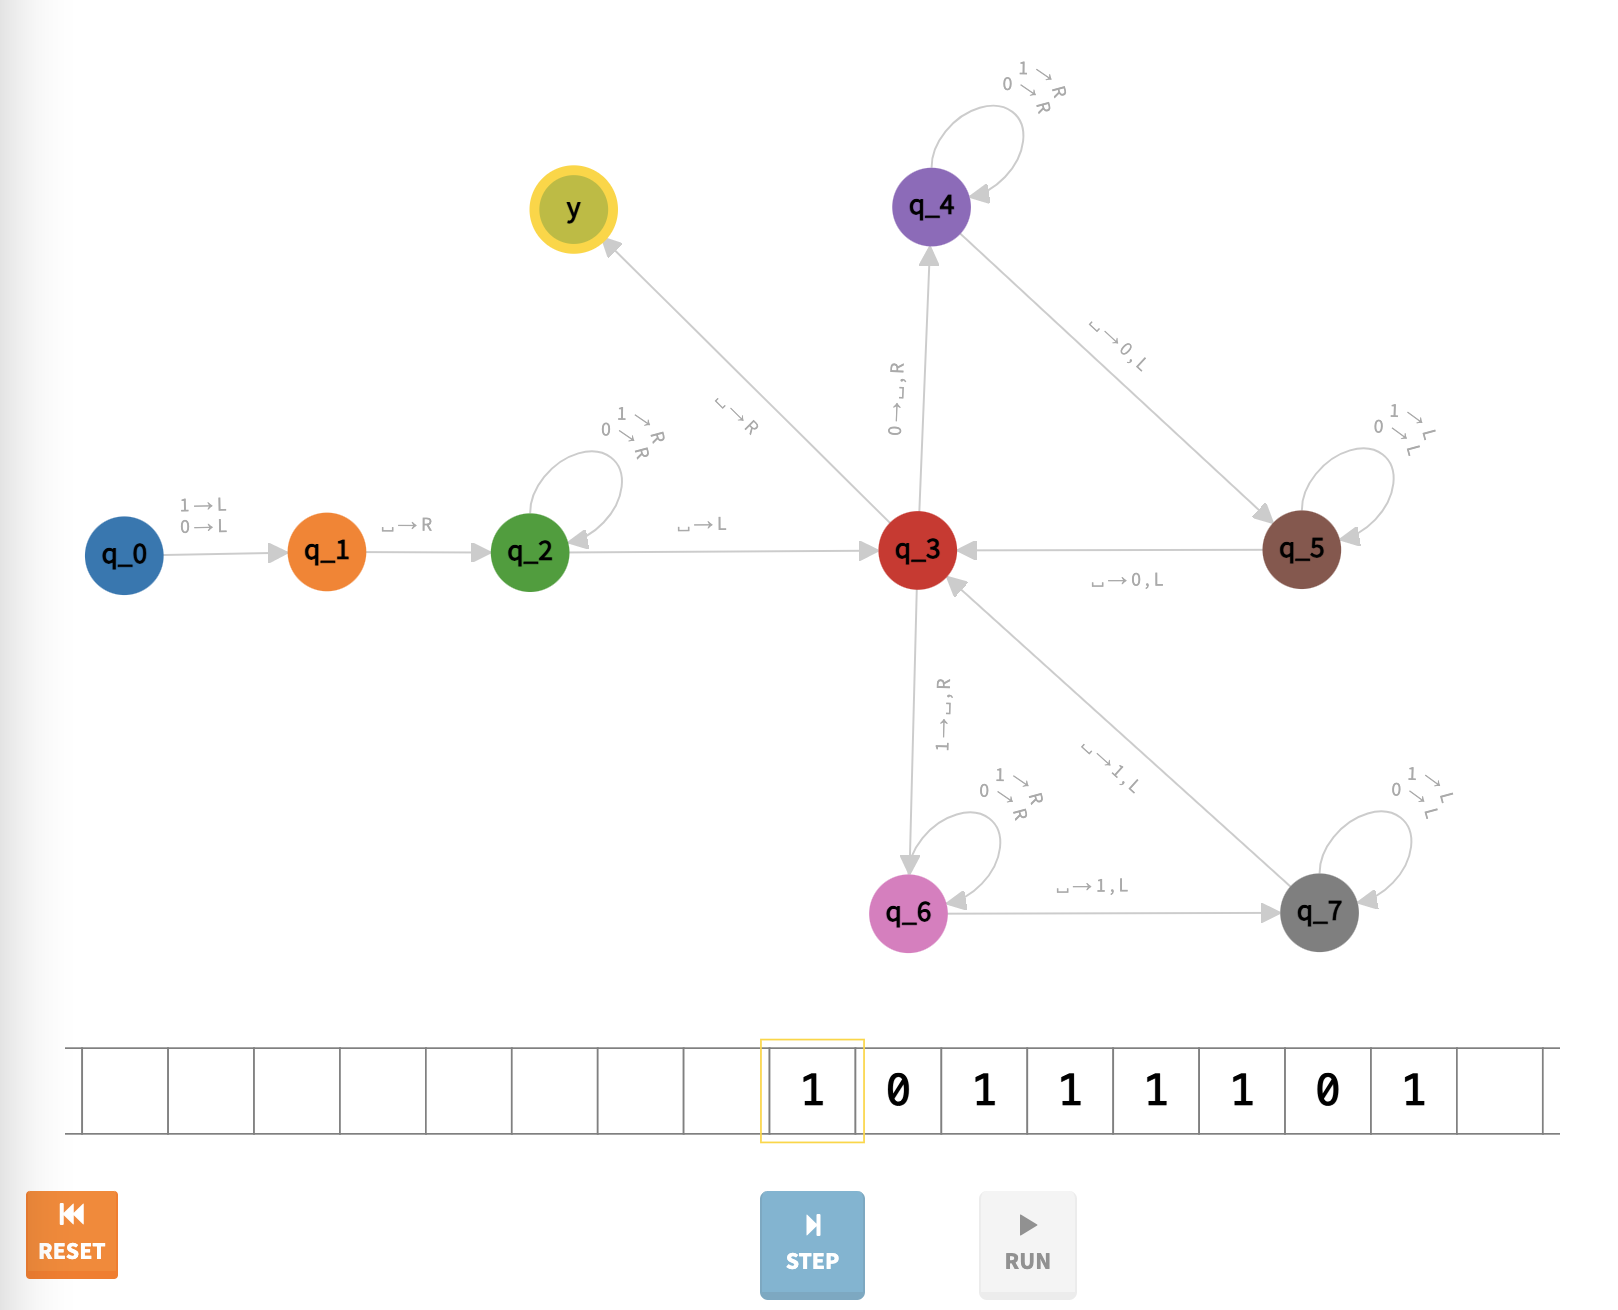
\includegraphics[width=\textwidth]{TM2.4}
\end{center}
\newpage
\begin{center}
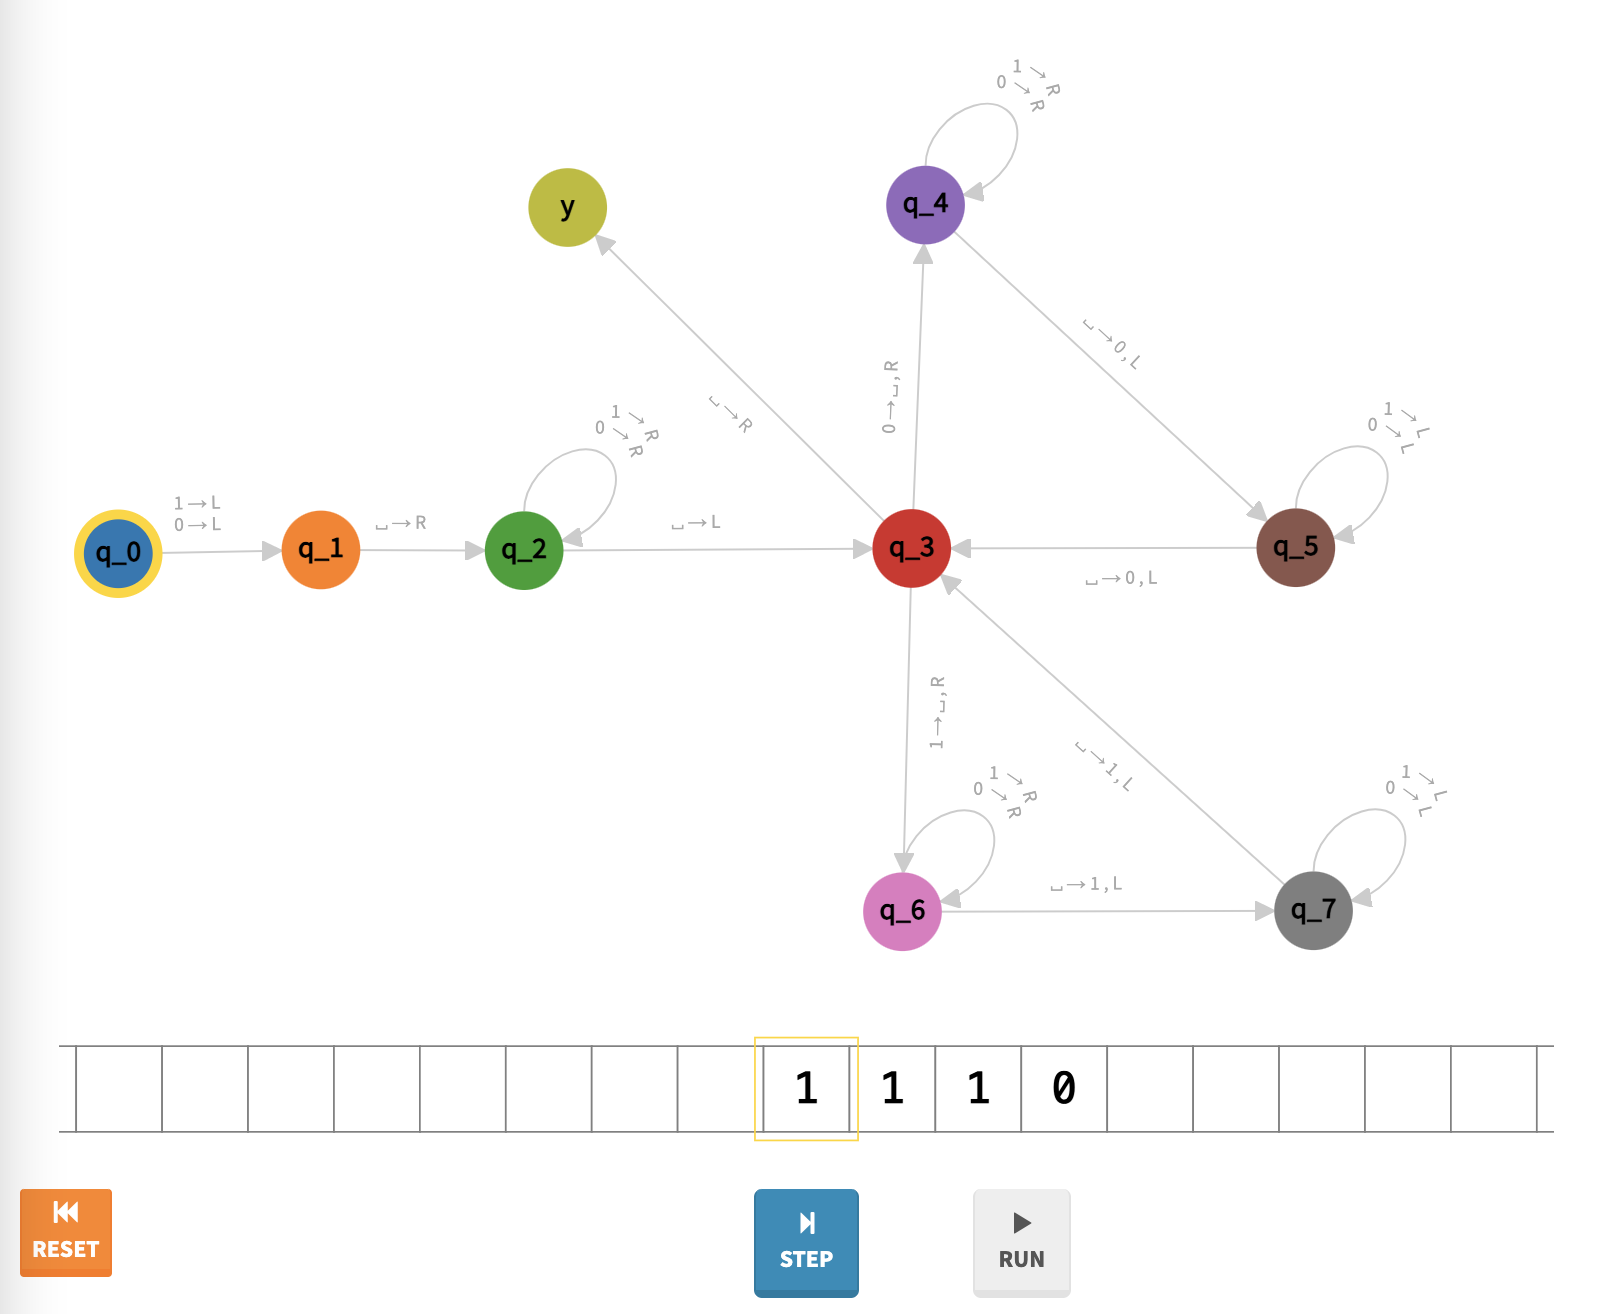
\includegraphics[width=\textwidth]{TM2.5}
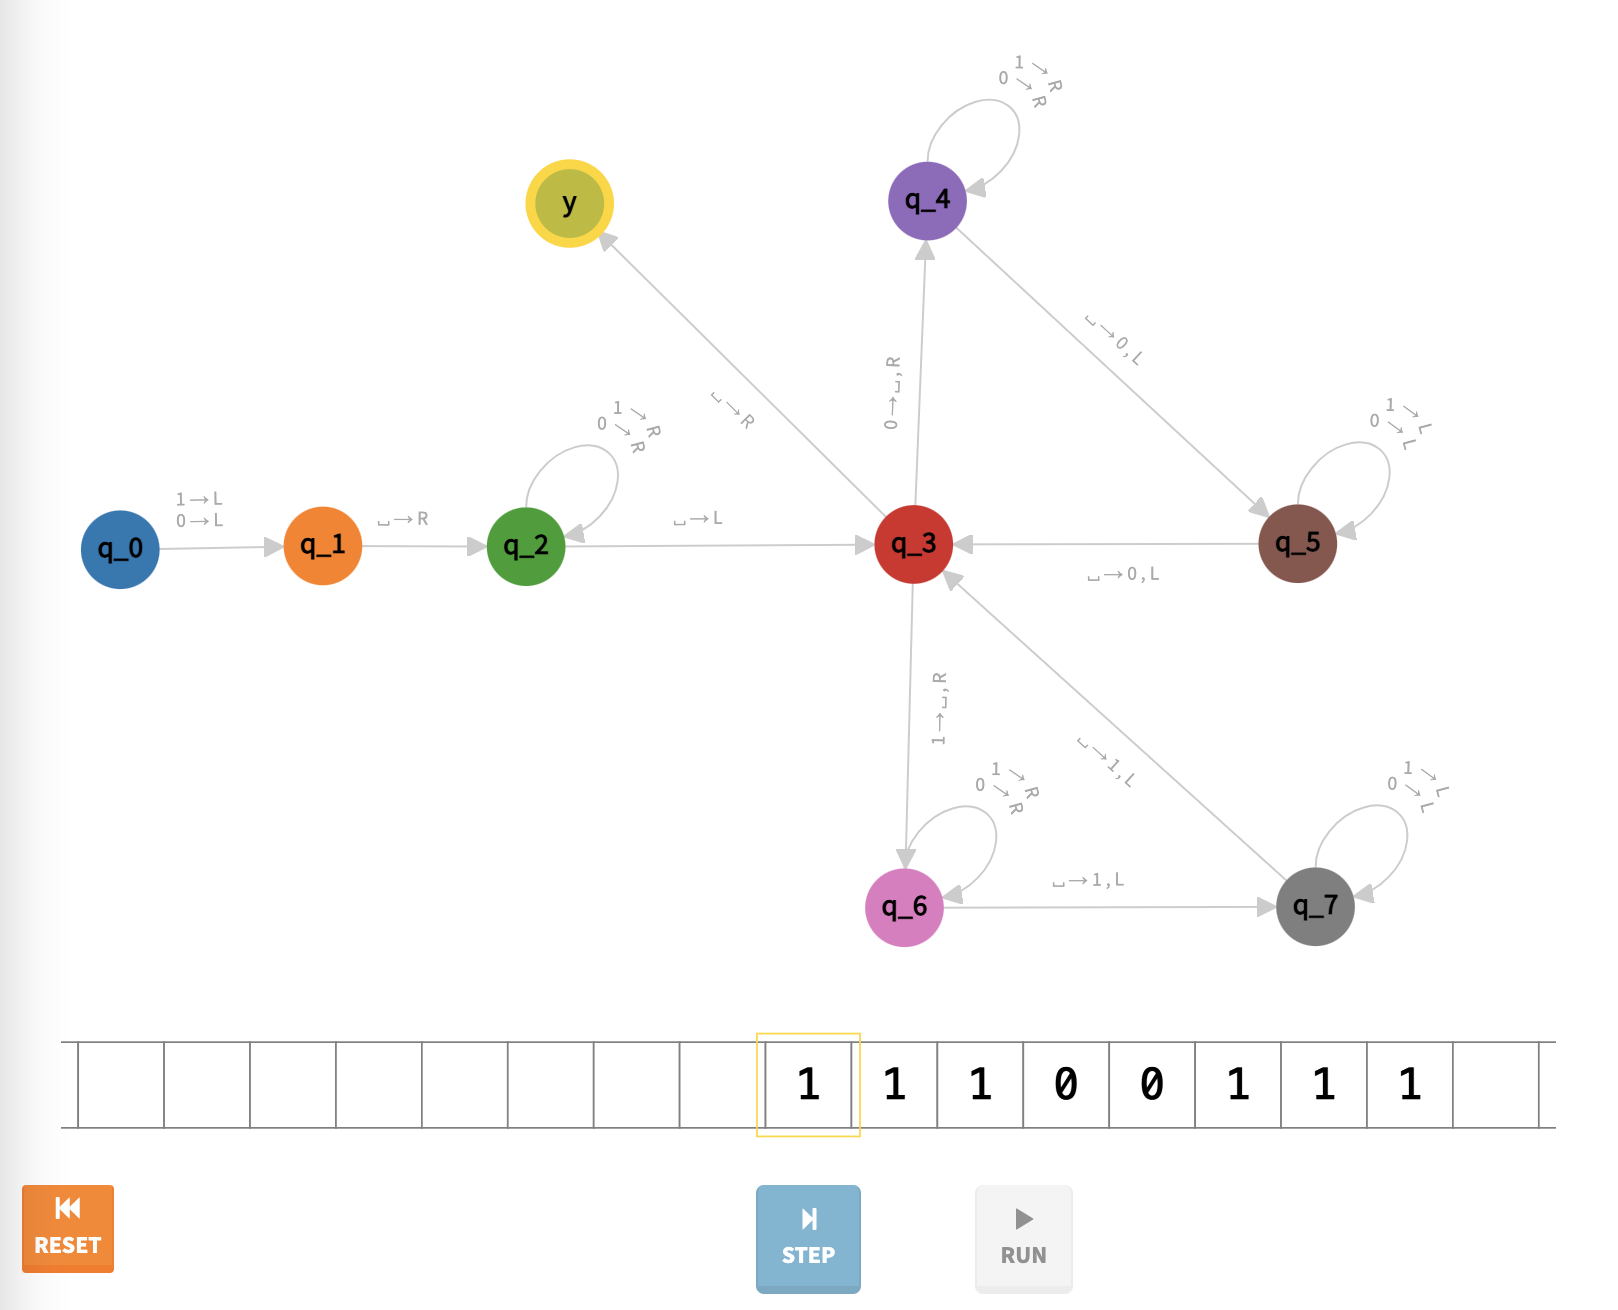
\includegraphics[width=\textwidth]{TM2.6}
\end{center}
\newpage
\begin{center}
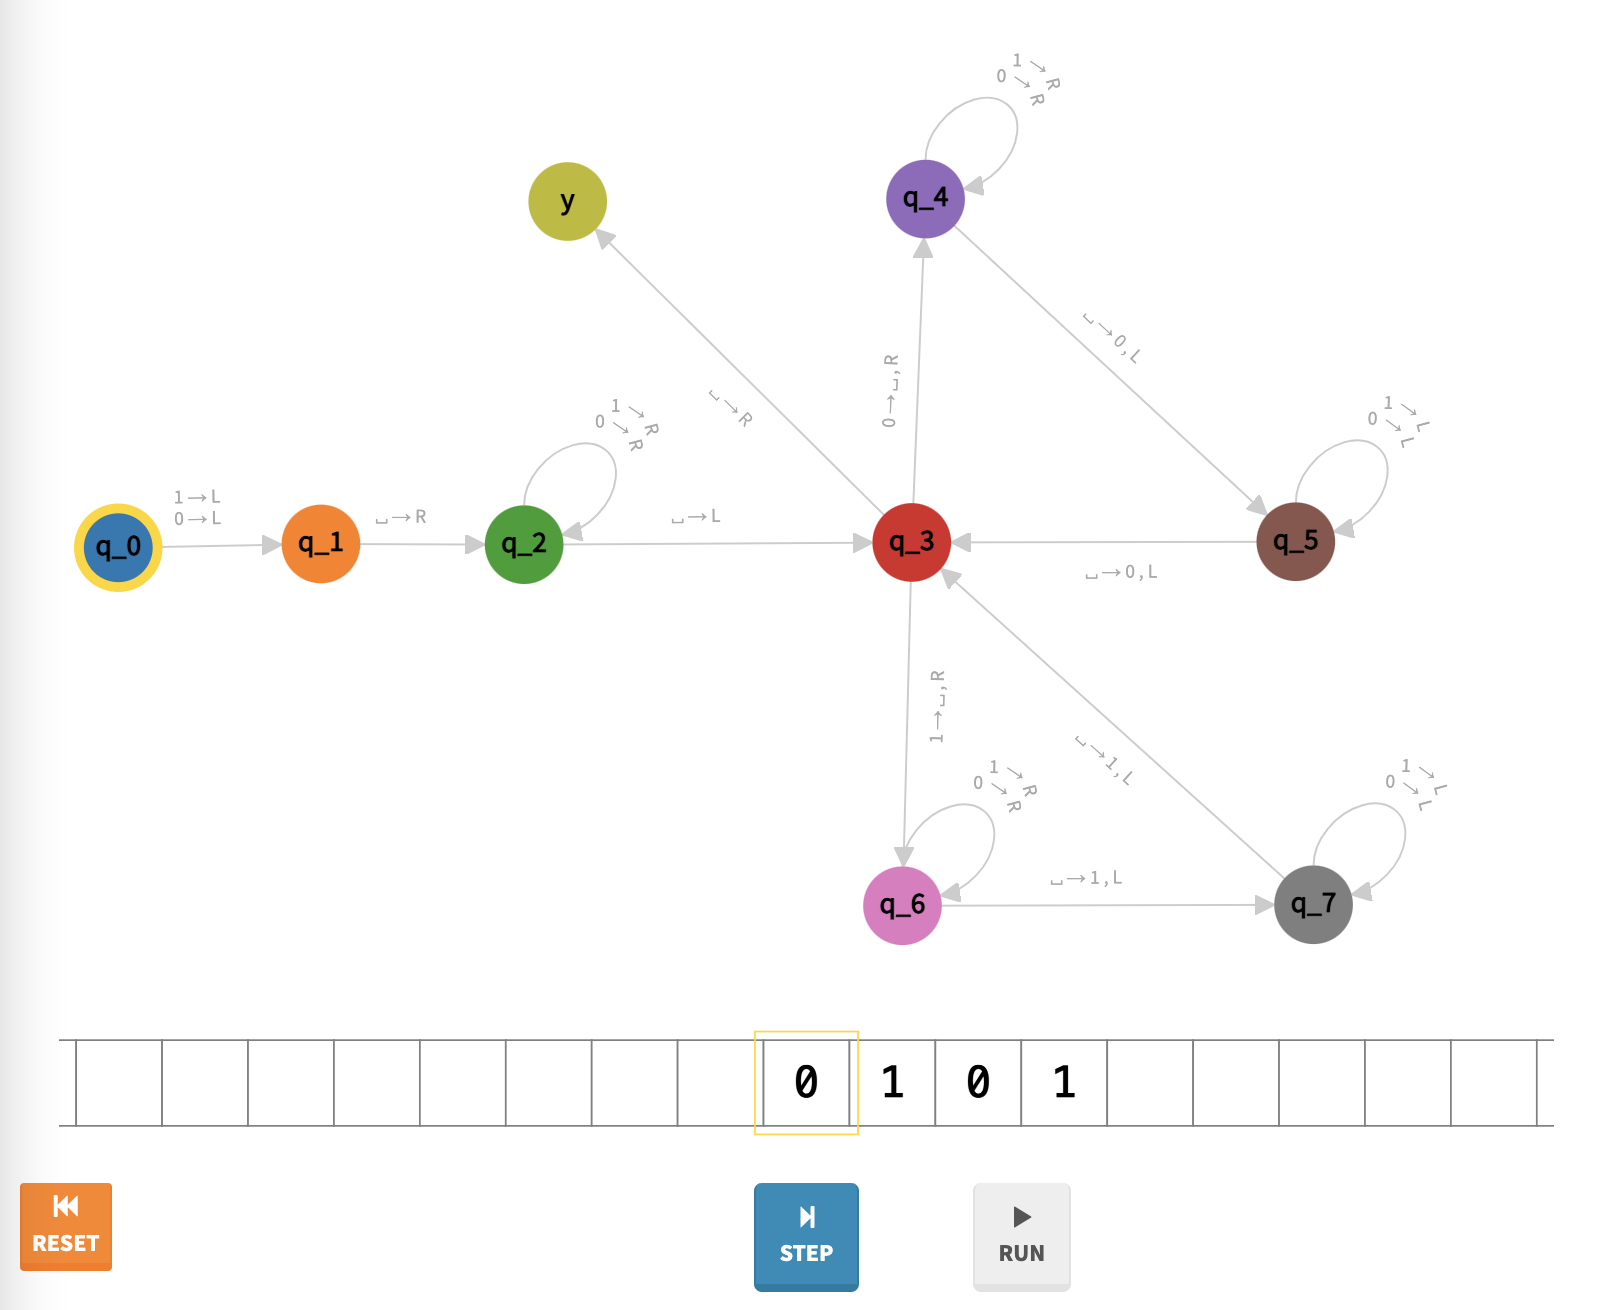
\includegraphics[width=\textwidth]{TM2.7}
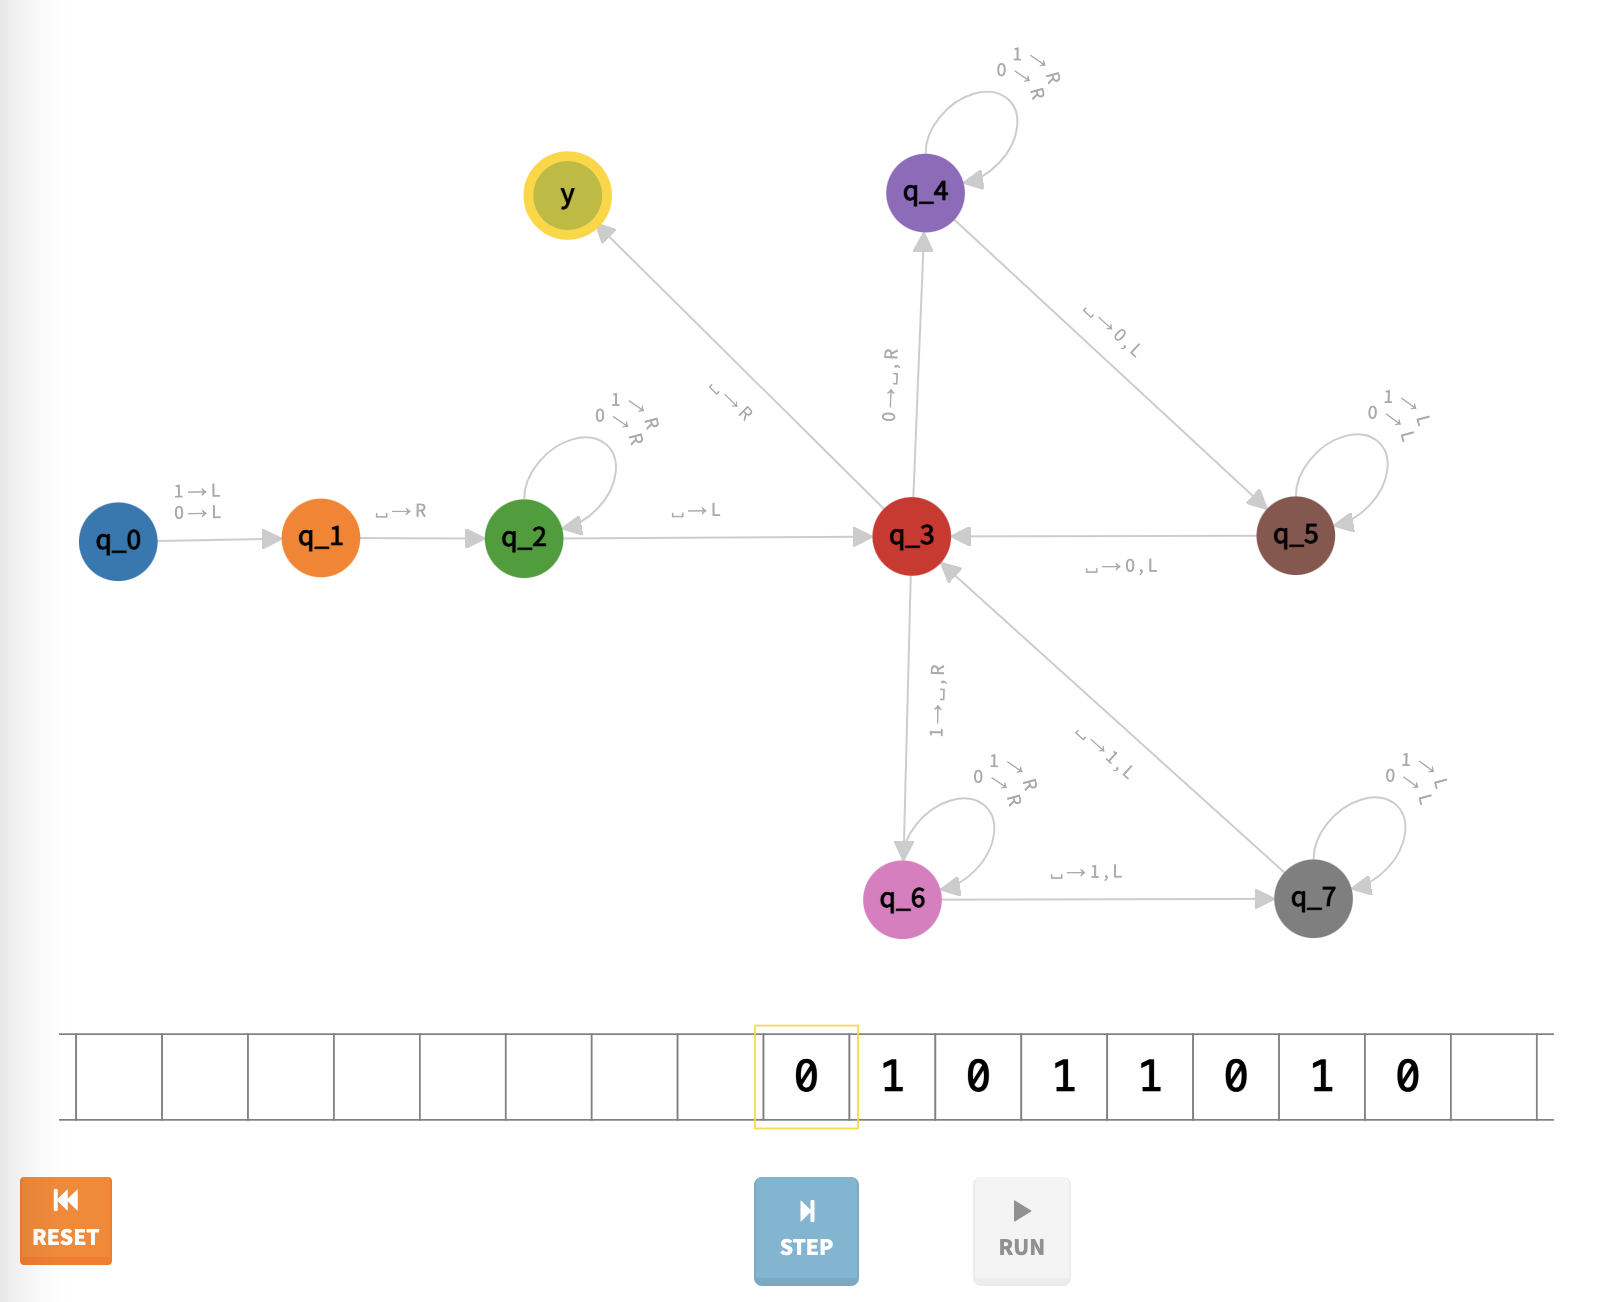
\includegraphics[width=\textwidth]{TM2.8}
\end{center}
\newpage
\begin{center}
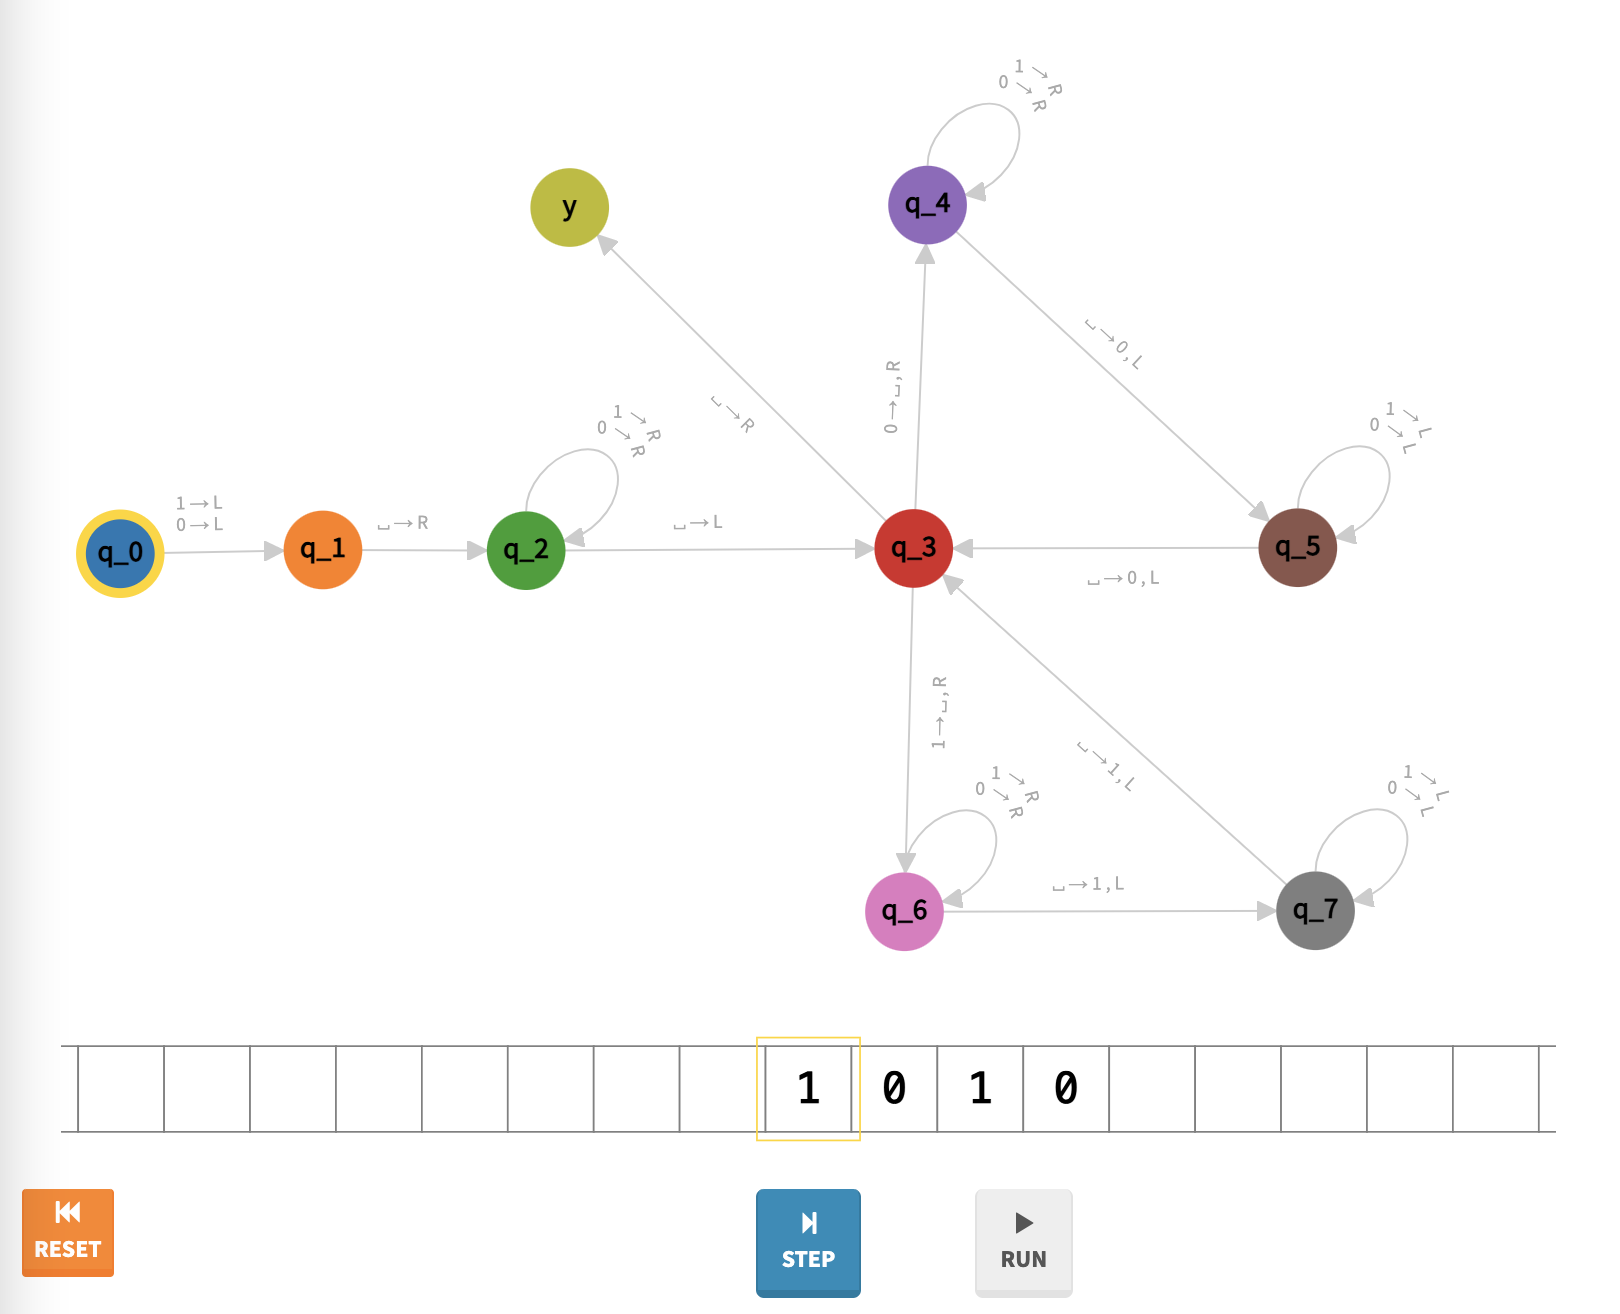
\includegraphics[width=\textwidth]{TM2.9}
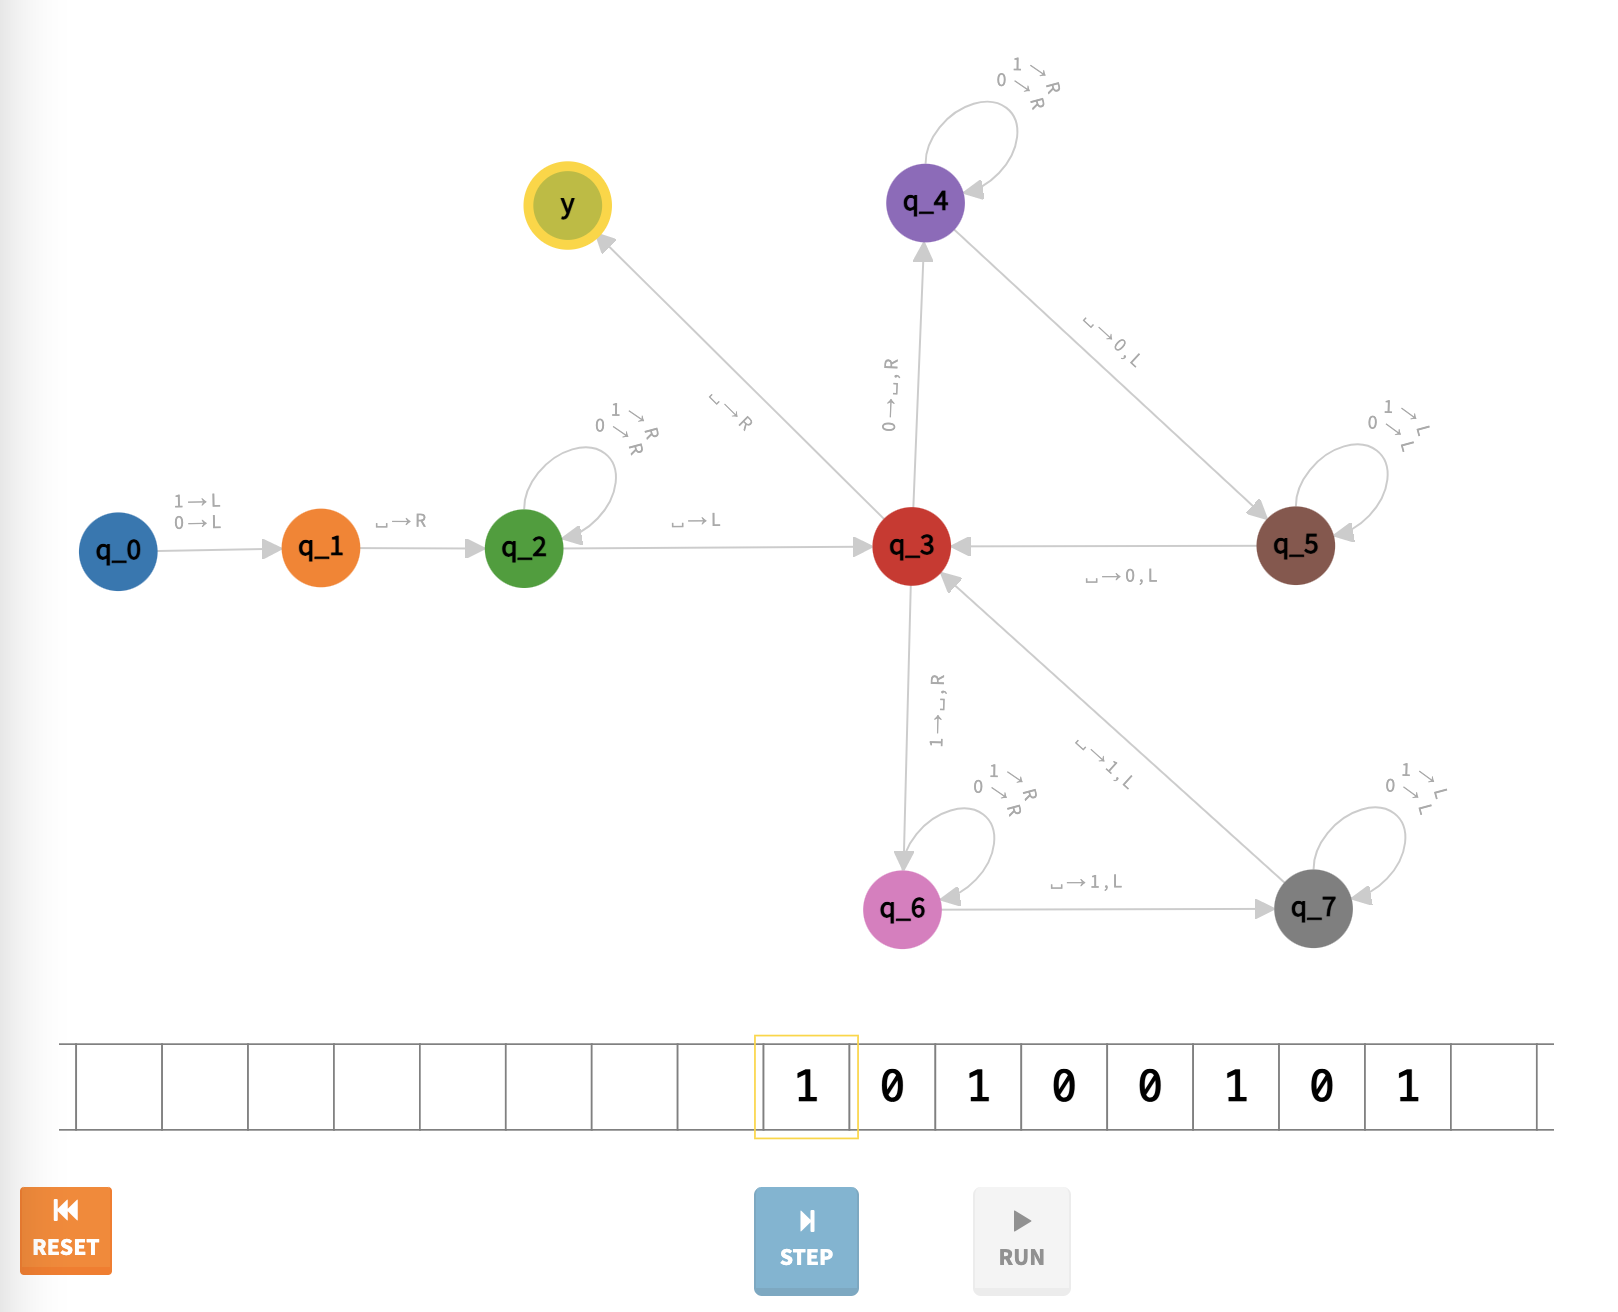
\includegraphics[width=\textwidth]{TM2.10}
\end{center}
\newpage
\begin{center}
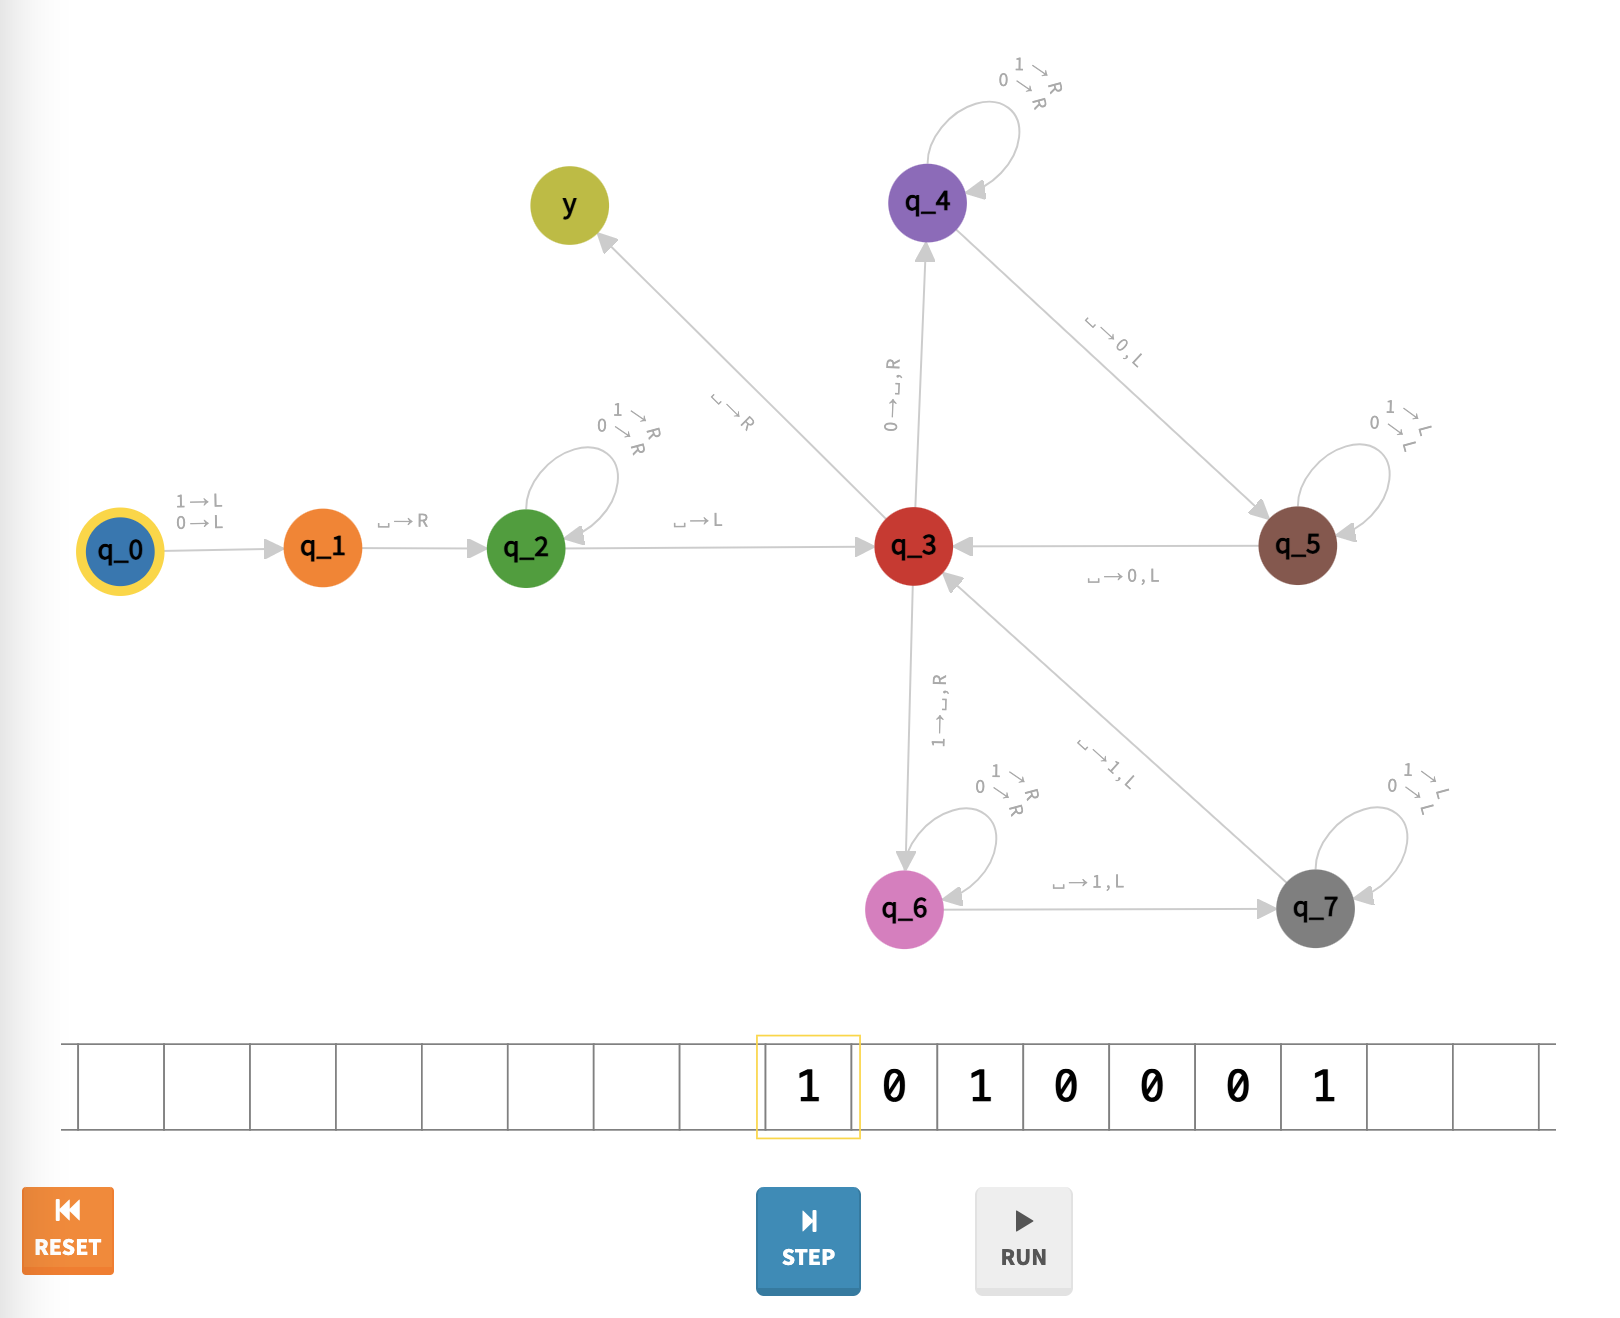
\includegraphics[width=\textwidth]{TM2.11}
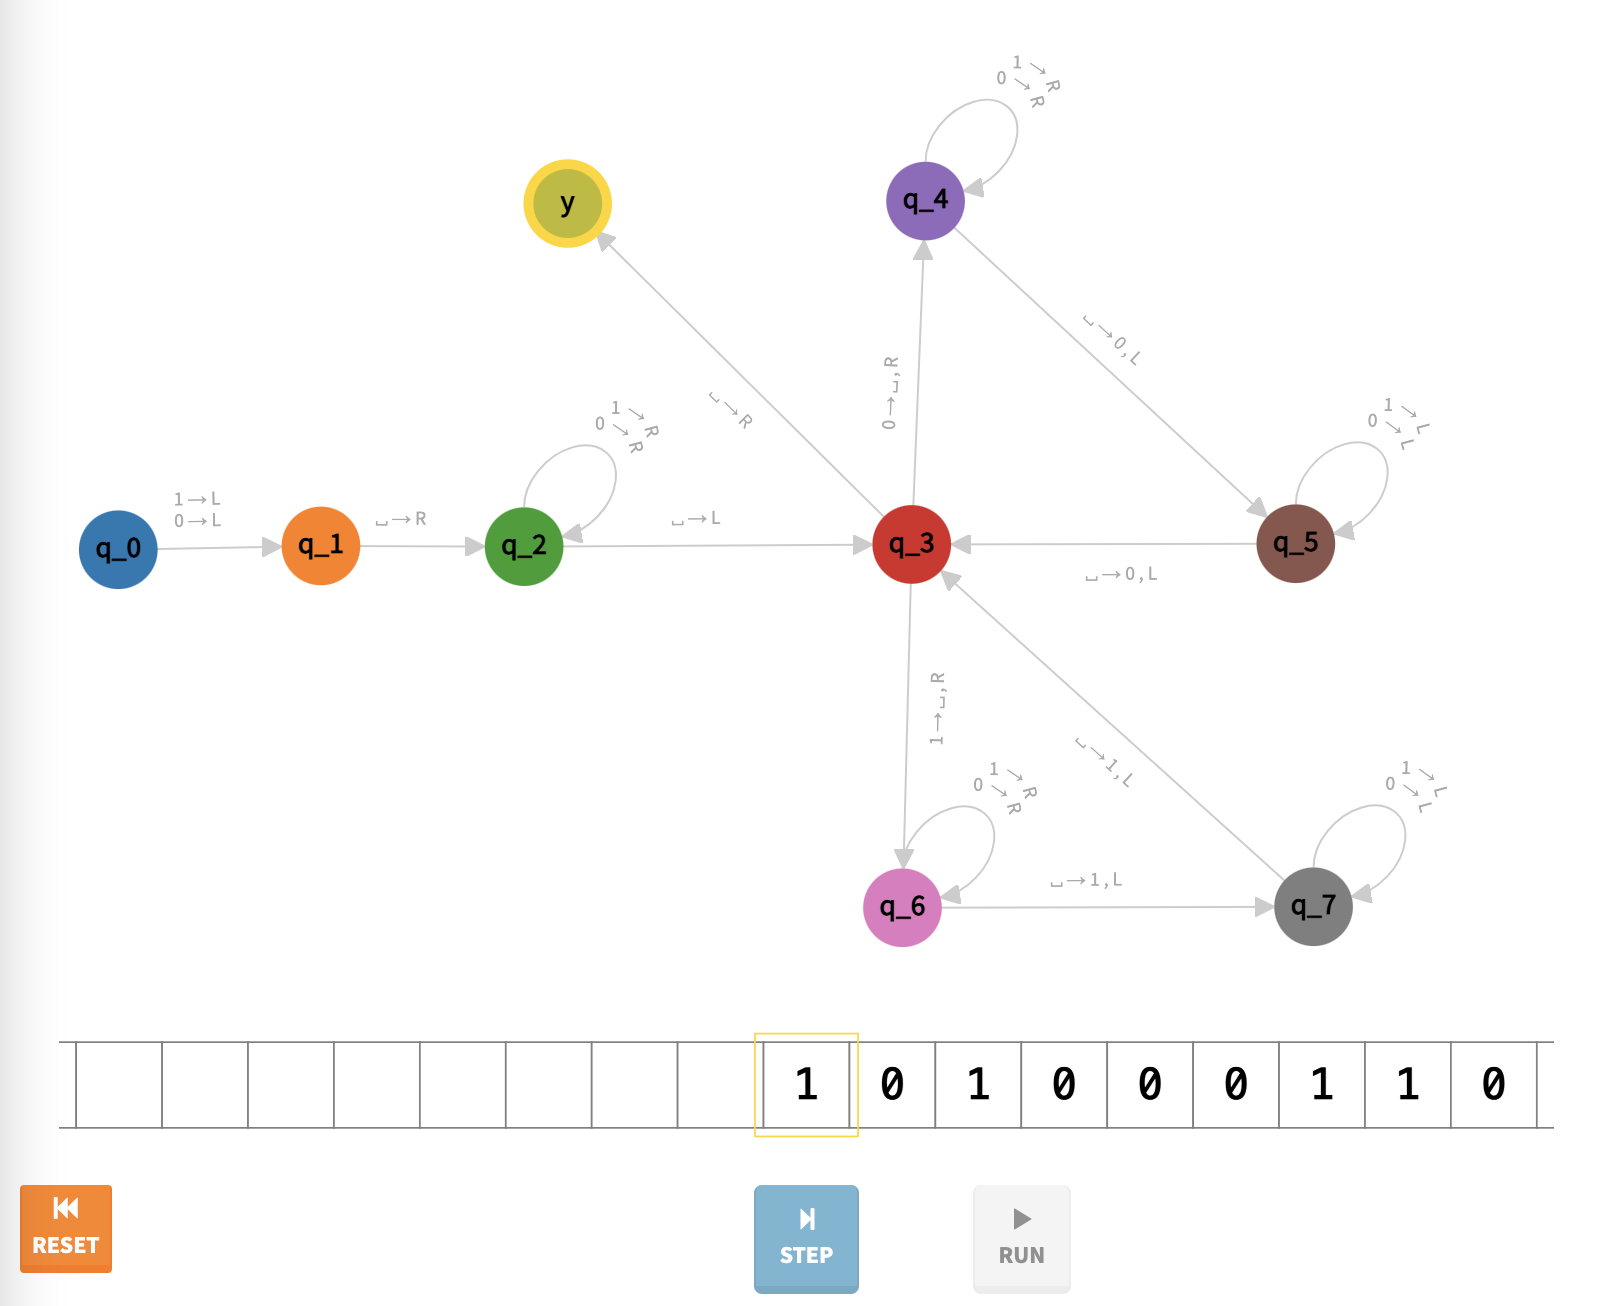
\includegraphics[width=\textwidth]{TM2.12}
\end{center}
\newpage
\begin{center}
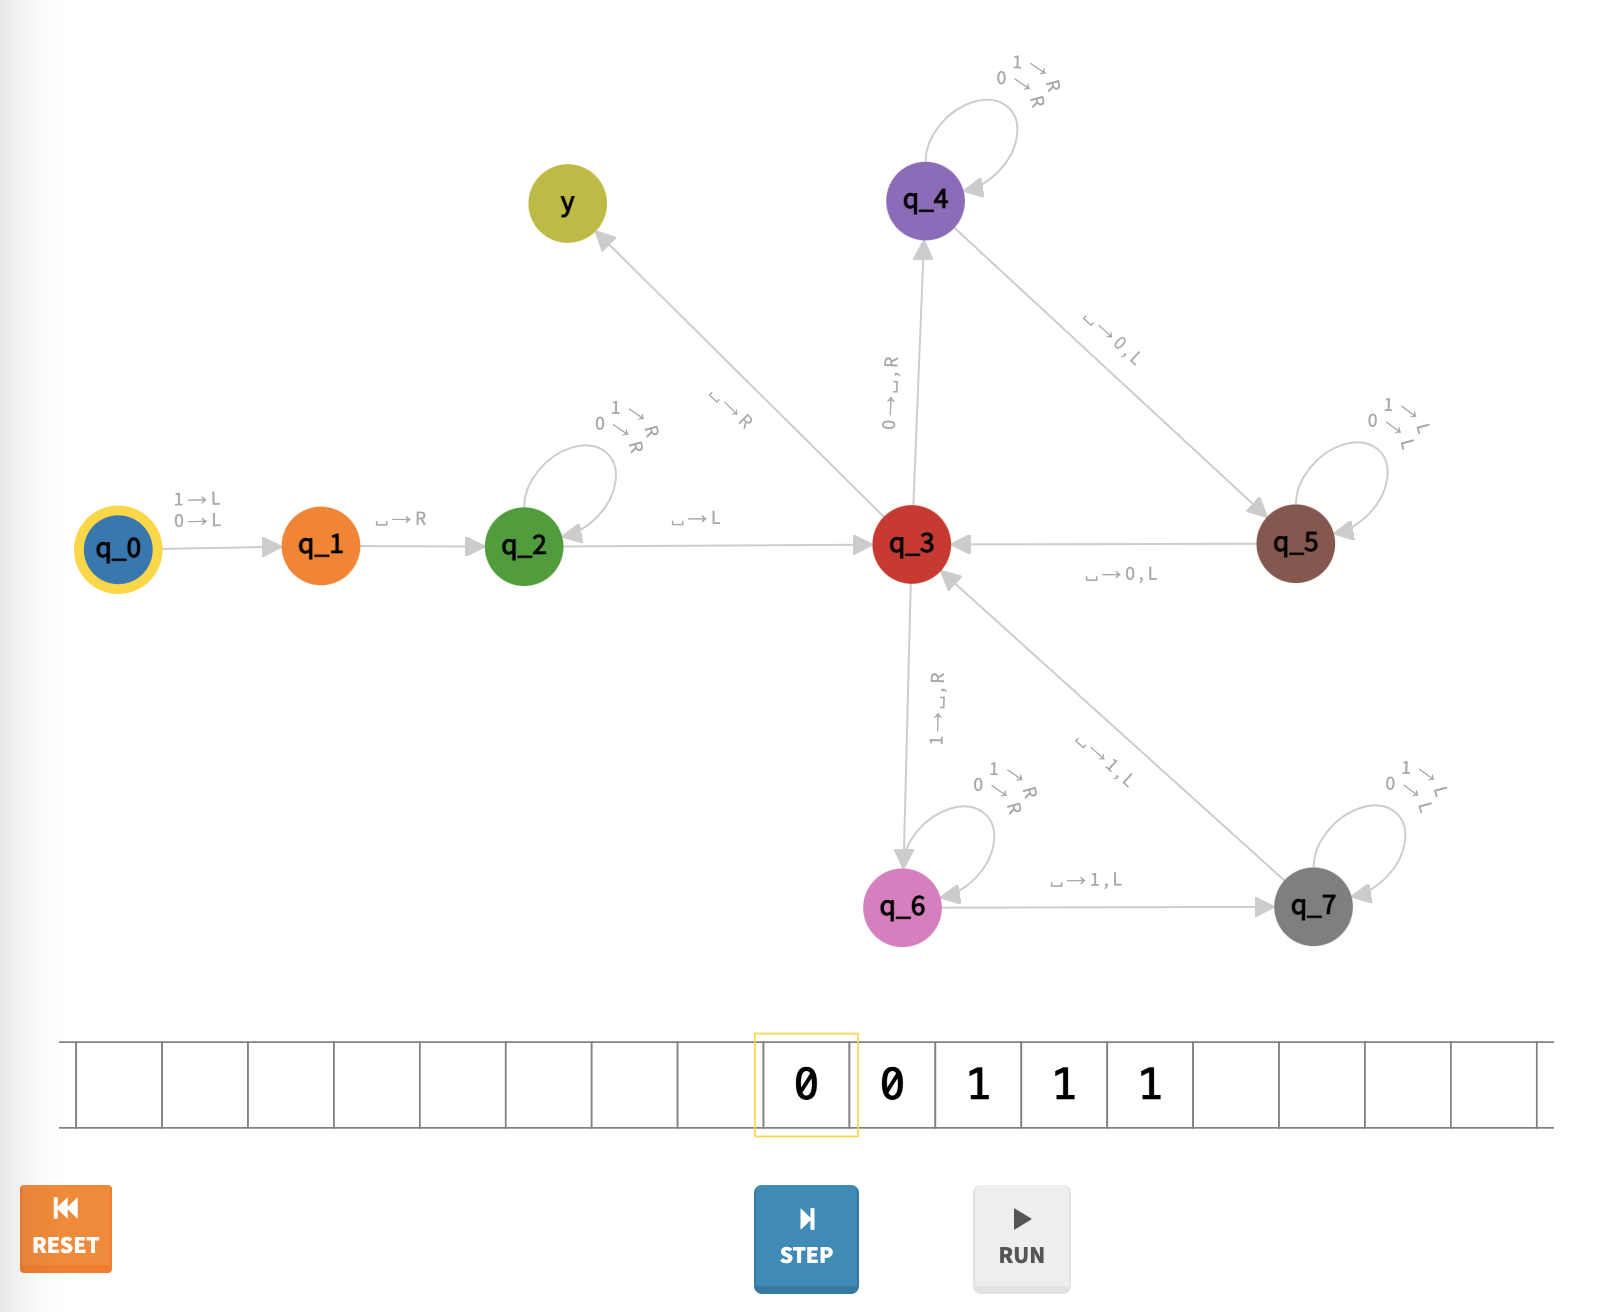
\includegraphics[width=\textwidth]{TM2.13}
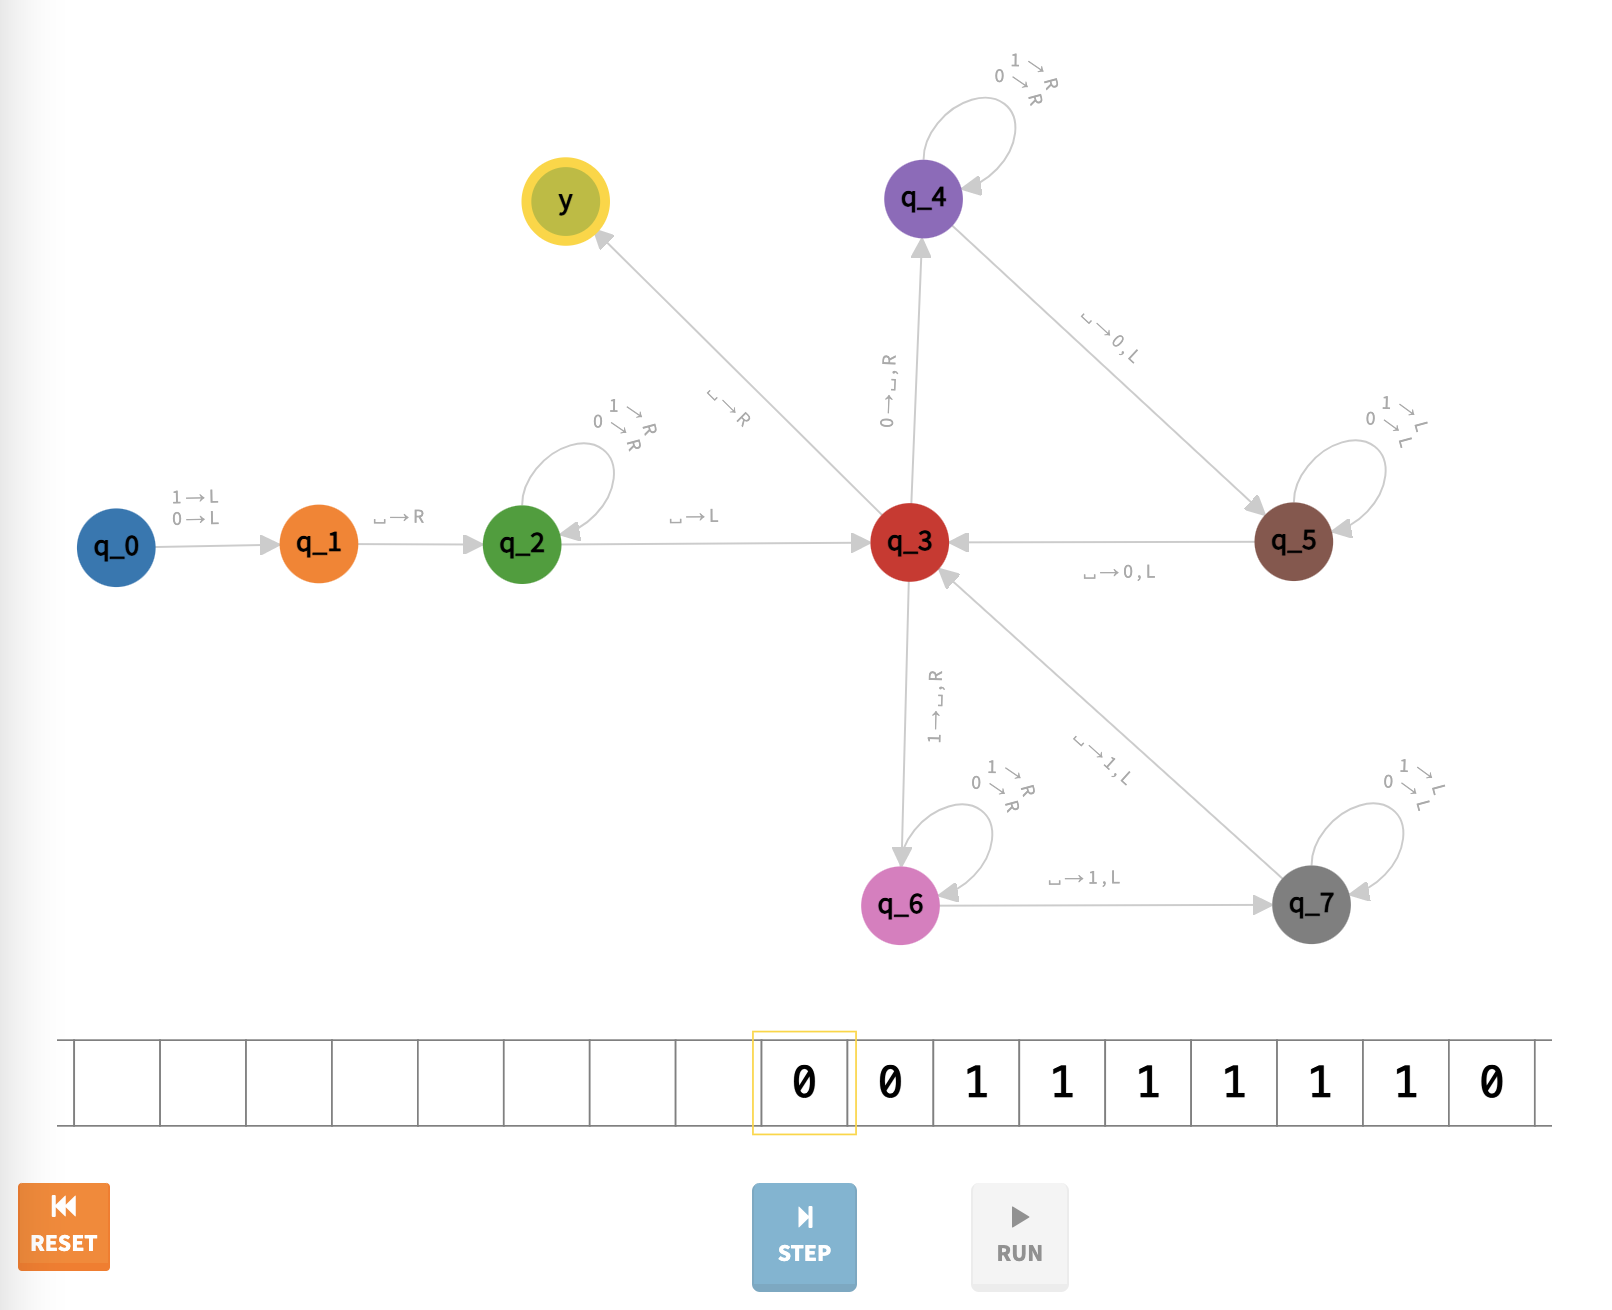
\includegraphics[width=\textwidth]{TM2.14}
\end{center}

\newpage

\section*{Answer 3}

Let $M$ be a Turing machine with a two-dimensional tape formally defined by the quintuple $(K, \Sigma, \delta, s, H)$ where $K$ is a finite set of states, $\Sigma$ is an alphabet, $\delta$ is the transition function, $s$ is the initial state, and $H$ is the set of halting states.
Let there be two more arrows, $\uparrow$ and $\downarrow$, which will denote the head moving up or down on the tape.
The tape goes to infinity for four sides, its center is marked with $\triangleright$ and it possesses similar properties with the usual $\triangleright$.
\begin{gather*}
\sqcup \in \Sigma,\ 
\triangleright \in \Sigma,\ 
\uparrow \notin \Sigma,\
\rightarrow \notin \Sigma,\ 
\downarrow \notin \Sigma,\
\leftarrow \notin \Sigma \\
\delta: \ (K \setminus H) \times \Sigma \ \rightarrow \ K \times (\Sigma \cup \{\uparrow, \rightarrow, \downarrow, \leftarrow\}) \\
\delta(q_0, \triangleright) = (q_1, p) \Rightarrow p = \rightarrow, \ \forall q_0 \in K \setminus H \\
\delta(q_0, p_0) = (q_1, p_1) \Rightarrow p_1 \neq \triangleright, \ \forall q_0 \in K \setminus H \land p_0 \in \Sigma \\
s \in K \\
H \subseteq K
\end{gather*}
\\
Each cell can be represented with a pair of integers.
Assume it is similar to a Cartesian coordinate system with pairs $(x,y)$ where $x$ increases in rightward direction and $y$ increases in upward direction.
Therefore a configuration for M is an element of $K \times \mathbb{Z} \times \mathbb{Z} \times F$ where $K$ is the set of states, $\mathbb{Z}$ is the set of integers, and $F$ is the set of all functions with the properties $f:\mathbb{Z} \times \mathbb{Z} \rightarrow \Sigma$ and $f(0,0)=\triangleright \ \forall f \in F$.
$F$ is defined in a way such that all elements of $F$ are functions with finitely many symbols different from $\sqcup$ in their ranges, more formally:
\begin{gather*}
\exists X \in \mathbb{Z},\ \forall y \in \mathbb{Z},\ \forall f \in F,\ (\lvert a \rvert > X \Rightarrow f(a,y) = \sqcup \land f(-a,y) = \sqcup) \\
\exists Y \in \mathbb{Z},\ \forall x \in \mathbb{Z},\ \forall f \in F,\ (\lvert a \rvert > Y \Rightarrow f(x, a) = \sqcup \land f(x,-a) = \sqcup)
\end{gather*}
$K$ represents the current state, $\mathbb{Z} \times \mathbb{Z}$ represent the position of the head, and $F$ represent the contents of the tape. \\
A step of computation, denoted with $(q_0, x_0, y_0, f_0) \vdash_M (q_1, x_1, y_1, f_1)$ is valid if and only if $\delta(q_0, f_0(x_0, y_0))=(q_1, p)$ and
\begin{align*}
p = \uparrow &\Leftrightarrow y_1 = y_0 + 1 \land x_1 = x_0 \land f_1 = f_0 \\
p = \rightarrow &\Leftrightarrow x_1 = x_0 + 1 \land y_1 = y_0 \land f_1 = f_0 \\
p = \downarrow &\Leftrightarrow y_1 = y_0 - 1 \land x_1 = x_0 \land f_1 = f_0 \\
p = \leftarrow &\Leftrightarrow x_1 = x_0 - 1 \land y_1 = y_0 \land f_1 = f_0 \\
p \notin \{\uparrow, \rightarrow, \downarrow, \leftarrow\} &\Leftrightarrow x_1 = x_0 \land y_1 = y_0 \land f_1(x_1, y_1) = p \\
\end{align*}
Let $\vdash^*_M$ be the reflexive transitive closure of $\vdash_M$.
The language accepted by this machine is as follows.
Let the machine $M$ have exactly two halting states, $y$ and $n$, and any other number of non-halting states.
Let $s$ be the starting state.
Let the string $w$ start from the position $(2,0)$ and go leftwards.
That is, $\forall i \in \mathbb{N},\ 2 \leq i \leq \lvert w \rvert + 2 \Rightarrow w_{i-2} = f(i, 0)$ where $f \in F$ is the function defining the contents of the tape.
Let the head start in the position $(1,0)$.
Let the machine $M$ halt for all inputs, that is, it is a decider, an algorithm.
The machine $M$ accepts this string if and only if it halts in the state $y$ and rejects otherwise.
More specifically:
\begin{gather*}
w \in L(M) \Leftrightarrow (s, 1, 0, F) \vdash^*_M (y, x_n, y_n, F_n)
\end{gather*}
Let $g: \mathbb{Z} \times \mathbb{Z} \rightarrow \mathbb{N}$ be a bijection mapping pairs of integers to natural numbers. Let $g(0,0)=0$. We can map the two-dimensional tape to a semi-infinite one-dimensional tape by using $g$. Let $M_s$ be the standard Turing machine with semi-infinite tape that will simulate $M$ which has a two-dimensional tape. Let $M_s$ be formally defined by the quintuple $(K_s, \Sigma_s, \delta_s, s_s, H_s)$, where
\begin{gather*}
K_s = K \\
\Sigma_s = \Sigma \\
\delta_s(q_0, p_0) = \delta(q_0, p_0) = (q_1, p_1) \Leftrightarrow p_1 \notin \{\uparrow, \rightarrow, \downarrow, \leftarrow\} \\
s_s = s \\
H_s = H \\
\end{gather*}
If $p_1 \in \{\uparrow, \rightarrow, \downarrow, \leftarrow\}$, then the machine $M_s$ moves the head to the appropriate position given by the function $g$. Therefore, the machine $M$ can be simulated by the standard Turing machine $M_s$.

\end{document}